%% For double-blind review submission, w/o CCS and ACM Reference (max submission space)
\documentclass[acmsmall,review,anonymous]{acmart}\settopmatter{printfolios=true,printccs=false,printacmref=false}
%% For double-blind review submission, w/ CCS and ACM Reference
%\documentclass[acmsmall,review,anonymous]{acmart}\settopmatter{printfolios=true}
%% For single-blind review submission, w/o CCS and ACM Reference (max submission space)
%\documentclass[acmsmall,review]{acmart}\settopmatter{printfolios=true,printccs=false,printacmref=false}
%% For single-blind review submission, w/ CCS and ACM Reference
%\documentclass[acmsmall,review]{acmart}\settopmatter{printfolios=true}
%% For final camera-ready submission, w/ required CCS and ACM Reference
%\documentclass[acmsmall]{acmart}\settopmatter{}

%% Journal information
%% Supplied to authors by publisher for camera-ready submission;
%% use defaults for review submission.
\acmJournal{PACMPL}
\acmVolume{1}
\acmNumber{ICFP}
\acmArticle{1}
\acmYear{2018}
\acmMonth{1}
\acmDOI{}
\startPage{1}

%% Copyright information
%% Supplied to authors (based on authors' rights management selection;
%% see authors.acm.org) by publisher for camera-ready submission;
%% use 'none' for review submission.
\setcopyright{none}
%\setcopyright{acmcopyright}
%\setcopyright{acmlicensed}
%\setcopyright{rightsretained}
%\copyrightyear{2018}           %% If different from \acmYear

\bibliographystyle{ACM-Reference-Format}
%% Note: author/year citations are required for papers published as an
%% issue of PACMPL.
\citestyle{acmauthoryear}

%%%%%%%%%%%%%%%%%%%%%%%%%%%%%%%%%%%%%%%%%%%%%%%%%%%%%%%%%%%%%%%%%%%%%%
%% Note: Authors migrating a paper from PACMPL format to traditional
%% SIGPLAN proceedings format must update the '\documentclass' and
%% topmatter commands above; see 'acmart-sigplanproc-template.tex'.
%%%%%%%%%%%%%%%%%%%%%%%%%%%%%%%%%%%%%%%%%%%%%%%%%%%%%%%%%%%%%%%%%%%%%%

\usepackage{bookmark}
\usepackage{booktabs}
\usepackage{subcaption}
\usepackage[utf8]{inputenc}
\usepackage[T1]{fontenc}
\usepackage{xspace}

% Haskell code snippets and useful shortcuts
\usepackage{minted}
\setminted[haskell]{escapeinside=@@}
\newcommand{\hs}{\mintinline{haskell}}
\newcommand{\cmd}[1]{\textsf{\color[rgb]{0,0,0.5} #1}}
\newcommand{\teq}{\smaller $\sim$}
\newcommand{\ghci}{$\lambda$>}
\newcommand{\defeq}{\stackrel{\text{def}}{=}}
\newcommand{\std}[1]{{\color[rgb]{0,0.3,0} #1}}
\newcommand{\blk}[1]{{\color[rgb]{0,0,0} #1}}

% Questions and tasks
\newcommand{\q}[2]{\textbf{\color{blue} Question #1:} #2}
\newcommand{\todo}[2]{\textbf{\color{red} #1:} #2}

% Abbreviations for build systems
\newcommand{\Make}{\textsc{Make}\xspace}
\newcommand{\Shake}{\textsc{Shake}\xspace}
\newcommand{\Ninja}{\textsc{Ninja}\xspace}
\newcommand{\Bazel}{\textsc{Bazel}\xspace}
\newcommand{\Buck}{\textsc{Buck}\xspace}
\newcommand{\CloudBuild}{\textsc{CloudBuild}\xspace}
\newcommand{\Nix}{\textsc{Nix}\xspace}
\newcommand{\Pluto}{\textsc{Pluto}\xspace}
\newcommand{\Excel}{\textsc{Excel}\xspace}
\newcommand{\Tup}{\textsc{Tup}\xspace}
\newcommand{\Fabricate}{\textsc{Fabricate}\xspace}
\newcommand{\Redo}{\textsc{Redo}\xspace}
\newcommand{\Calc}{\textsc{Calc}\xspace}
\newcommand{\store}{\hs{k}~\hs{->}~\hs{v}\xspace}
\newcommand{\storef}{\hs{k}~\hs{->}~\hs{f}~\hs{v}\xspace}

\begin{document}

%% [Short title] Title
\title[Build Systems \`a la Carte]{Build Systems \`a la Carte}
% \titlenote{with title note}
% \subtitle{Subtitle}
% \subtitlenote{with subtitle note}

%% Author information
%% Contents and number of authors suppressed with 'anonymous'.
%% Each author should be introduced by \author, followed by
%% \authornote (optional), \orcid (optional), \affiliation, and
%% \email.
%% An author may have multiple affiliations and/or emails; repeat the
%% appropriate command.
%% Many elements are not rendered, but should be provided for metadata
%% extraction tools.

%% Author with single affiliation.
\author{First1 Last1}
\authornote{with author1 note}          %% \authornote is optional;
                                        %% can be repeated if necessary
\orcid{nnnn-nnnn-nnnn-nnnn}             %% \orcid is optional
\affiliation{
  \position{Position1}
  \department{Department1}              %% \department is recommended
  \institution{Institution1}            %% \institution is required
  \streetaddress{Street1 Address1}
  \city{City1}
  \state{State1}
  \postcode{Post-Code1}
  \country{Country1}                    %% \country is recommended
}
\email{first1.last1@inst1.edu}          %% \email is recommended

%% Author with two affiliations and emails.
\author{First2 Last2}
\authornote{with author2 note}          %% \authornote is optional;
                                        %% can be repeated if necessary
\orcid{nnnn-nnnn-nnnn-nnnn}             %% \orcid is optional
\affiliation{
  \position{Position2a}
  \department{Department2a}             %% \department is recommended
  \institution{Institution2a}           %% \institution is required
  \streetaddress{Street2a Address2a}
  \city{City2a}
  \state{State2a}
  \postcode{Post-Code2a}
  \country{Country2a}                   %% \country is recommended
}
\email{first2.last2@inst2a.com}         %% \email is recommended
\affiliation{
  \position{Position2b}
  \department{Department2b}             %% \department is recommended
  \institution{Institution2b}           %% \institution is required
  \streetaddress{Street3b Address2b}
  \city{City2b}
  \state{State2b}
  \postcode{Post-Code2b}
  \country{Country2b}                   %% \country is recommended
}
\email{first2.last2@inst2b.org}         %% \email is recommended

\begin{abstract}
Build systems are awesome. Build systems are terrifying. In this paper ...
\end{abstract}

%% 2012 ACM Computing Classification System (CSS) concepts
%% Generate at 'http://dl.acm.org/ccs/ccs.cfm'.
\begin{CCSXML}
<ccs2012>
<concept>
<concept_id>10011007.10011006.10011008</concept_id>
<concept_desc>Software and its engineering~General programming languages</concept_desc>
<concept_significance>500</concept_significance>
</concept>
<concept>
<concept_id>10003456.10003457.10003521.10003525</concept_id>
<concept_desc>Social and professional topics~History of programming languages</concept_desc>
<concept_significance>300</concept_significance>
</concept>
</ccs2012>
\end{CCSXML}

\ccsdesc[500]{Software and its engineering~General programming languages}
\ccsdesc[300]{Social and professional topics~History of programming languages}
%% End of generated code

% \keywords{functional programming, build systems}

\maketitle

\section{Introduction}\label{sec-intro}

Build systems (such as \Make) are big, complicated, and used by every
software developer on the planet.  But they are a sadly unloved part
of the software ecosystem, very much a means to an end, and seldom the
focus of attention.
% Rarely do people ask questions like ``What does it mean for my build
% system to be correct?'' or ``What are the trade-offs between different
% approaches?''.
For years \Make dominated, but more recently the challenges of scale have driven
large software firms like Microsoft, Facebook and Google to develop their own
build systems, exploring new points in the design space. These complex build
systems use subtle algorithms, but they are often hidden away, and not the
object of study.

In this paper we give a general framework in which to understand and compare
build systems, in a way that is both abstract (omitting incidental detail) and
yet precise (implemented as Haskell code). Specifically we make these
contributions:

\begin{itemize}
\item Build systems vary on many axes, including: static vs dynamic
  dependencies; local vs cloud; deterministic vs non-deterministic build tasks;
  early cutoff; self-tracking build systems; and the type of persistently stored
  build information. In~\S\ref{sec-background} we identify some of these key
  properties, illustrated by four carefully-chosen build systems.

\item We describe some simple but novel abstractions that
  crisply encapsulate what a build system is (\S\ref{sec-abstractions}),
  allowing us, for example, to speak about what it means for a build system to
  be correct.

\item We identify two key design choices that are typically deeply wired into
  any build system: \emph{the order in which tasks are
  built}~(\S\ref{sec-scheduler}) and \emph{whether or not a
  task is rebuilt}~(\S\ref{sec-rebuilder}). These choices turn out to
  be orthogonal, which leads us to a new classification of the design
  space~(\S\ref{sec-design-space}).

\item We show that we can instantiate our abstractions to describe the essence
of a variety of different real-life build systems, including \Make, \Shake,
\Bazel, \Buck, \Nix, and \Excel\footnote{\Excel appears very different to the
others but, seen through the lens of this paper, it is very close.}, each by the
composition of the two design choices~(\S\ref{sec-implementations}). Doing this
modelling in a single setting allows the differences and similarities between
these huge systems to be brought out clearly\footnote{All our models are
executable and are available on Hackage as \cmd{build-1.0}.}.

\item Moreover, we can readily remix the ingredients to design new build systems
with desired properties, for example, to combine the advantages of \Shake and
\Bazel. Writing this paper gave us the insights to combine dynamic dependencies
and cloud build systems in a principled way; we evaluate the result
in~\S\ref{sec-experience}.

\item We can use the presented abstractions to more clearly explain details from
the original \Shake paper~(\S\ref{sec-step-traces}, \S\ref{sec-experience-shake})
and develop new cloud build features, which are already in use in industry and in
the GHC build system~(\S\S\ref{sec-using-cloud-shake}-\ref{sec-hadrian}).

\end{itemize}

In short, instead of seeing build systems as unrelated points in space, we now
see them as locations in a connected landscape, leading to a better
understanding of what they do and how they compare, and making it easier to
explore other points in the landscape. While we steer clear of many engineering
aspects of real build systems, in~\S\ref{sec-engineering} we discuss these
aspects in the context of the presented abstractions. The related work is covered
in~\S\ref{sec-related}.

This paper is an extended version of an earlier conference
paper~\cite{mokhov2018buildsystems}. The key changes compared to the earlier
version are: (i) we added further clarifications and examples
to~\S\ref{sec-abstractions}, in particular,~\S\ref{sec-task-examples} is
entirely new; (ii)~\S\ref{sec-scheduler} and~\S\ref{sec-rebuilder} are based on
the material from the conference paper but have been substantially expanded to
include further details and examples, as well as completely new material such
as~\S\ref{sec-step-traces}; (iii)~\S\ref{sec-experience} is completely new; (iv)
\S\ref{sec-failures} and \S\S\ref{sec-polymorphism}-\ref{sec-file-watching}
are almost entirely new, and \S\ref{sec-non-determinism} has been revised.
The new material focuses on our experience and various important practical
considerations, hence justifying the ``and Practice'' part of the paper title.

\section{Background}\label{sec-background}

Build systems automate the execution of repeatable tasks for individual users
and large organisations. In this section we explore the design space of build
systems, using four concrete examples: \Make~\cite{feldman1979make},
\Shake~\cite{mitchell2012shake}, \Bazel~\cite{bazel}, and
\Excel~\cite{advanced_excel}.
We have carefully chosen these four to illustrate the various axes on which
build systems differ; we discuss many other notable examples of build systems,
and their relationships, in~\S\ref{sec-implementations} and~\S\ref{sec-related}.

\subsection{The venerable \Make: static dependencies and file modification times}
\label{sec-background-make}

\Make\footnote{There are numerous implementations of \Make and none comes with a
formal specification. In this paper we therefore use a simple and sensible
approximation to a real \Make that you might find on your machine.} was developed
more than 40 years ago to automatically build software libraries and executable
programs from source code. It uses \emph{makefiles} to describe tasks (often
referred to as \emph{build rules}) and their dependencies in a simple textual form.
For example:

\vspace{1mm}
\begin{minted}[xleftmargin=10pt]{makefile}
util.o: util.h util.c
    gcc -c util.c
\end{minted}
\vspace{1mm}
\begin{minted}[xleftmargin=10pt]{makefile}
main.o: util.h main.c
    gcc -c main.c
\end{minted}
\vspace{1mm}
\begin{minted}[xleftmargin=10pt]{makefile}
main.exe: util.o main.o
    gcc util.o main.o -o main.exe
\end{minted}
\vspace{1mm}

\noindent
The above makefile lists three tasks: (i) compile a utility library comprising
files \cmd{util.h} and \cmd{util.c} into \cmd{util.o} by
executing\footnote{In this example we pretend \cmd{gcc} is a pure function for
the sake of simplicity. In reality, there are multiple versions of \cmd{gcc};
the actual binary used to compile and link files, and standard libraries
such that \cmd{stdio.h}, are often also listed as dependencies.} the command
\cmd{gcc -c util.c}, (ii) compile the main source file \cmd{main.c} into
\cmd{main.o}, and (iii) link object files \cmd{util.o} and \cmd{main.o} into the
executable \cmd{main.exe}. The makefile contains the complete information about
the \emph{task dependency graph}, which is shown in Fig.~\ref{fig-make}(a).

\begin{figure}[h]
\begin{subfigure}[b]{0.32\linewidth}
\centerline{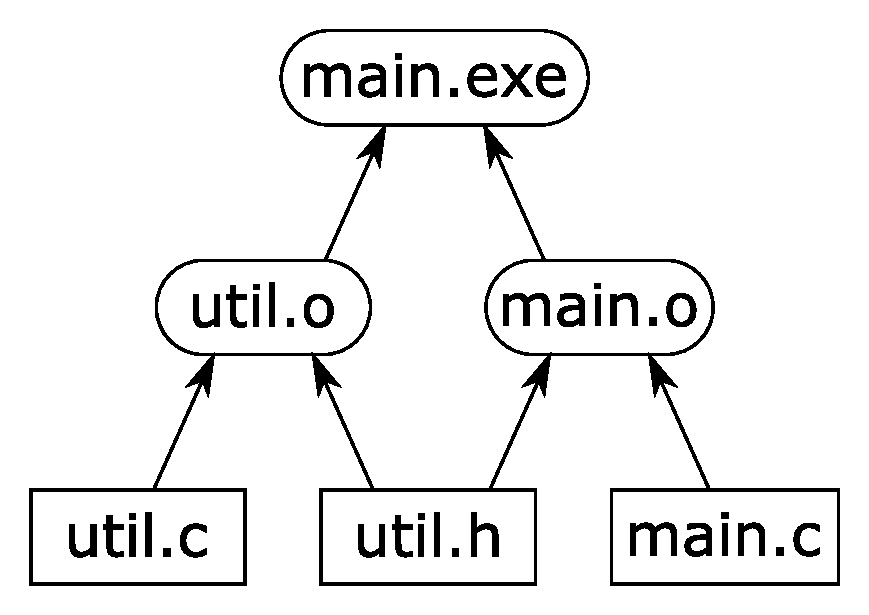
\includegraphics[scale=0.28]{fig/make-example.pdf}}
\caption{Task dependency graph}
\end{subfigure}
\begin{subfigure}[b]{0.32\linewidth}
\centerline{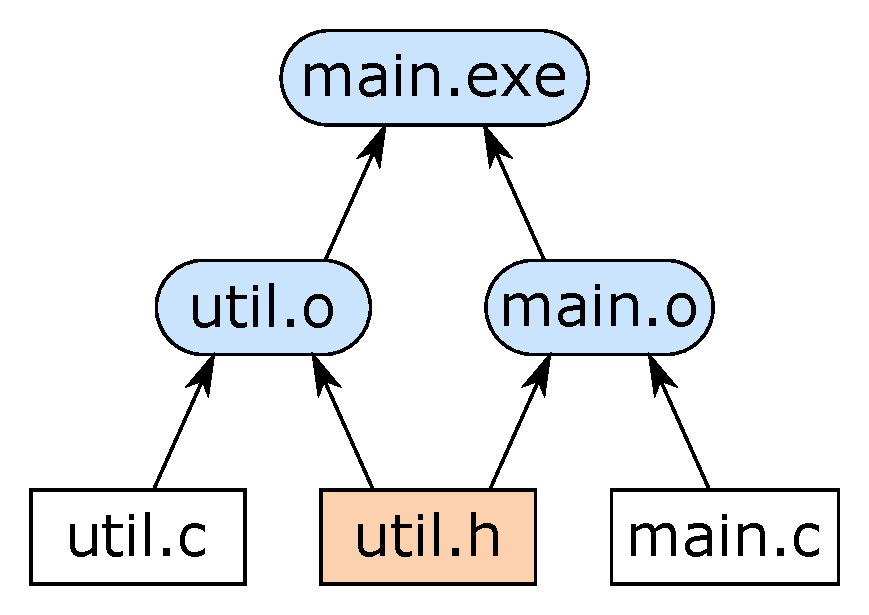
\includegraphics[scale=0.28]{fig/make-example-full.pdf}}
\caption{Full rebuild}
\end{subfigure}
\begin{subfigure}[b]{0.32\linewidth}
\centerline{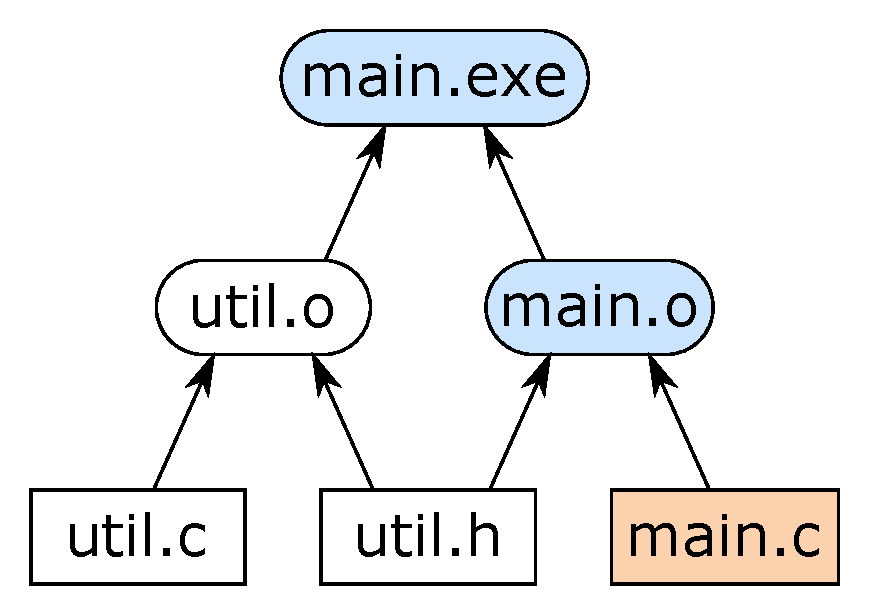
\includegraphics[scale=0.28]{fig/make-example-partial.pdf}}
\caption{Partial rebuild}
\end{subfigure}
\vspace{-2mm}
\caption{A task dependency graph and two build scenarios. Input files are shown
in rectangles, intermediate and output files are shown in rounded rectangles.
Modified inputs and files that are rebuilt are highlighted.
\label{fig-make}}
\vspace{-2mm}
\end{figure}

If the user runs \Make specifying \cmd{main.exe} as the desired output, \Make
will build~\cmd{util.o}~and~\cmd{main.o}, in any order since these tasks are
independent, and then \cmd{main.exe}. If the user modifies \cmd{util.h} and runs
\Make again, it will perform a \emph{full rebuild}, because all three tasks
transitively depend on \cmd{util.h}, as illustrated in Fig.~\ref{fig-make}(b).
On the other hand, if the user modifies \cmd{main.c} then a \emph{partial
rebuild} is sufficient: \cmd{util.o} does not need to be rebuilt, since its
inputs have not changed, see Fig.~\ref{fig-make}(c). Note that if the dependency
graph is \emph{acyclic} then each task needs to be executed at most once. Cyclic
task dependencies are typically not allowed in build systems but there are rare
exceptions, see~\S\ref{sec-iterative-compute}.

\noindent
The following property is essential for build systems; indeed, it is their
raison d'\^etre:

\definition[Minimality]{A build system is \emph{minimal} if it executes tasks at
most once per build and only if they transitively depend on inputs that changed
since the previous build.}\label{def-minimal}
\vspace{2mm}

To achieve minimality \Make relies on two main ideas: (i) it uses \emph{file
modification times} to detect which files changed\footnote{Technically, you
can fool \Make by altering the modification time of a file without changing its
content, e.g. by using the command \cmd{touch}. \Make is therefore minimal only
under the assumption that you do not do that.}, and (ii) it constructs a task
dependency graph from the information contained in the makefile and executes
tasks in a \emph{topological order}. For a more concrete description
see~\S\ref{sec-implementation-make}.

\subsection{\Excel: dynamic dependencies at the cost of minimality}
\label{sec-background-excel}

\Excel is a build system in disguise. Consider the following simple spreadsheet.

\vspace{1mm}
\begin{minted}[xleftmargin=10pt]{text}
A1: 10      B1: A1 + A2
A2: 20
\end{minted}
\vspace{1mm}

\noindent
There are two input cells \cmd{A1} and \cmd{A2}, and a single task that computes
the sum of their values, producing the result in cell \cmd{B1}. If either of
the inputs change, \Excel will recompute the result.

Unlike \Make, \Excel does not need to know all task dependencies upfront. Indeed, some
dependencies may change \emph{dynamically} according to computation results. For
example:

\vspace{1mm}
\begin{minted}[xleftmargin=10pt]{text}
A1: 10      B1: INDIRECT("A" & C1)      C1: 1
A2: 20
\end{minted}
\vspace{1mm}

\noindent
The formula in \cmd{B1} uses the \cmd{INDIRECT} function, which takes a string
and returns the value of the cell with that name.  The string evaluates to
\cmd{"A1"}, so \cmd{B1} evaluates to \cmd{10}. However, the dependencies of the
formula in \cmd{B1} are determined by the value of \cmd{C1}, so it is impossible
to compute the dependency graph before the build starts\footnote{In
this particular example one might say that the value of
\cmd{C1} is statically known, but imagine that it is the result of a long
computation chain -- its value will only become available during the build.}.

To support dynamic dependencies, \Excel's calc engine~\cite{excel_recalc} is
significantly different from \Make. \Excel arranges the cells into a linear
sequence, called the \emph{calc chain}.  During the build, \Excel processes
cells in the calc-chain sequence, but if computing a cell \cmd{C} requires the
value of a cell \cmd{D} that has not yet been computed, \Excel \emph{aborts}
computation of \cmd{C}, moves \cmd{D} before \cmd{C} in the calc chain, and
resumes the build starting with \cmd{D}. When a build is complete, the resulting
calc chain respects all the dynamic dependencies of the spreadsheet. When an
input value (or formula) is changed, \Excel uses the final calc chain from the
\emph{previous} build as its starting point so that, in the common case where
changing an input value does not change dependencies, there are no aborts.
Notice that build always succeeds regardless of the initial calc chain (barring
truly circular dependencies); the calc chain is just an optimisation.
We refer to this algorithm as \emph{restarting}, and discuss it
in more detail in~\S\ref{sec-implementation-excel}.

Dynamic dependencies complicate minimality.  In the above example, \cmd{B1}
should only be recomputed if \cmd{A1} or \cmd{C1} change, but not if (say)
\cmd{A2} changes; but these facts are not statically apparent. In practice
\Excel implements a conservative approximation to minimality: it recomputes a
formula if~(i)~the formula statically mentions a changed cell, or~(ii)~the formula uses a
function like \cmd{INDIRECT} whose dependencies are not statically visible,
or~(iii)~the formula itself has changed.

Item (iii) in the above list highlights another distinguishing feature of \Excel: it
is \emph{self-tracking}. Most build systems only track changes of inputs and
intermediate results, but \Excel also tracks changes in the tasks themselves: if
a formula is modified, \Excel will recompute it and propagate the changes.
Self-tracking is uncommon in software build systems, where one often needs to
manually initiate a full rebuild even if just a single task has changed.
We discuss self-tracking further in~\S\ref{sec-tracking-aspects}.

\begin{figure}
\begin{subfigure}[b]{0.90\linewidth}
\centerline{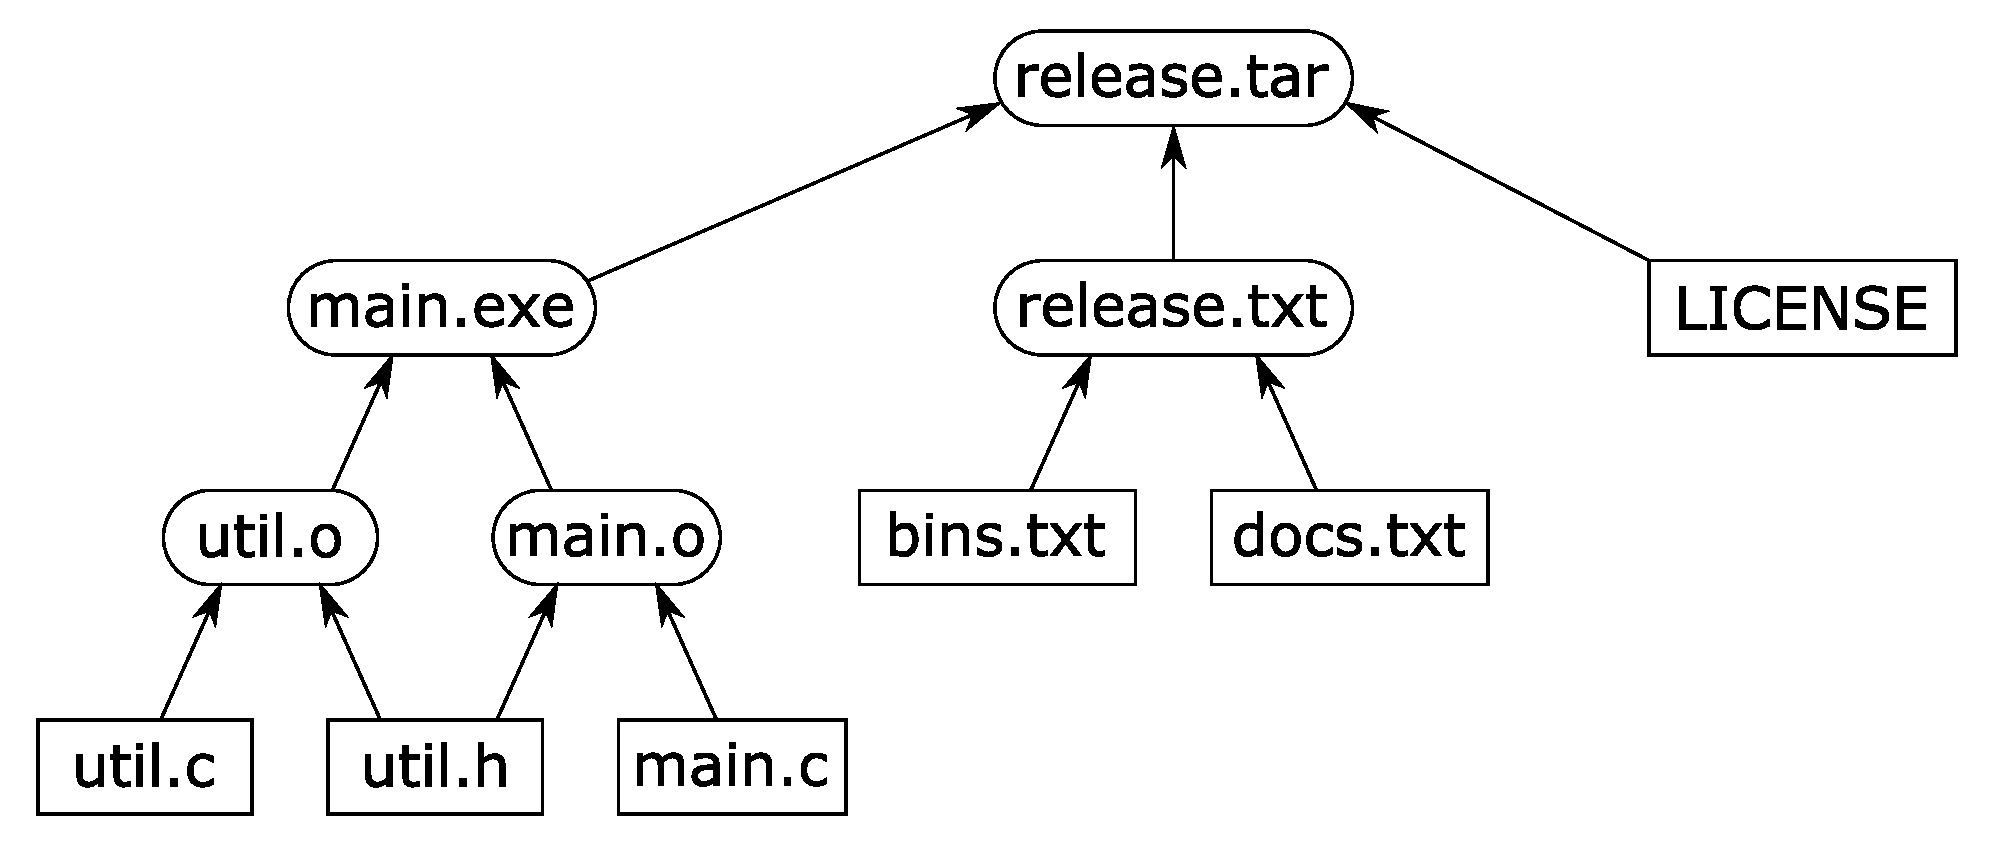
\includegraphics[scale=0.28]{fig/shake-example.pdf}}
\caption{Dependency graph produced after the previous build.}
\end{subfigure}
\begin{subfigure}[b]{0.90\linewidth}
\centerline{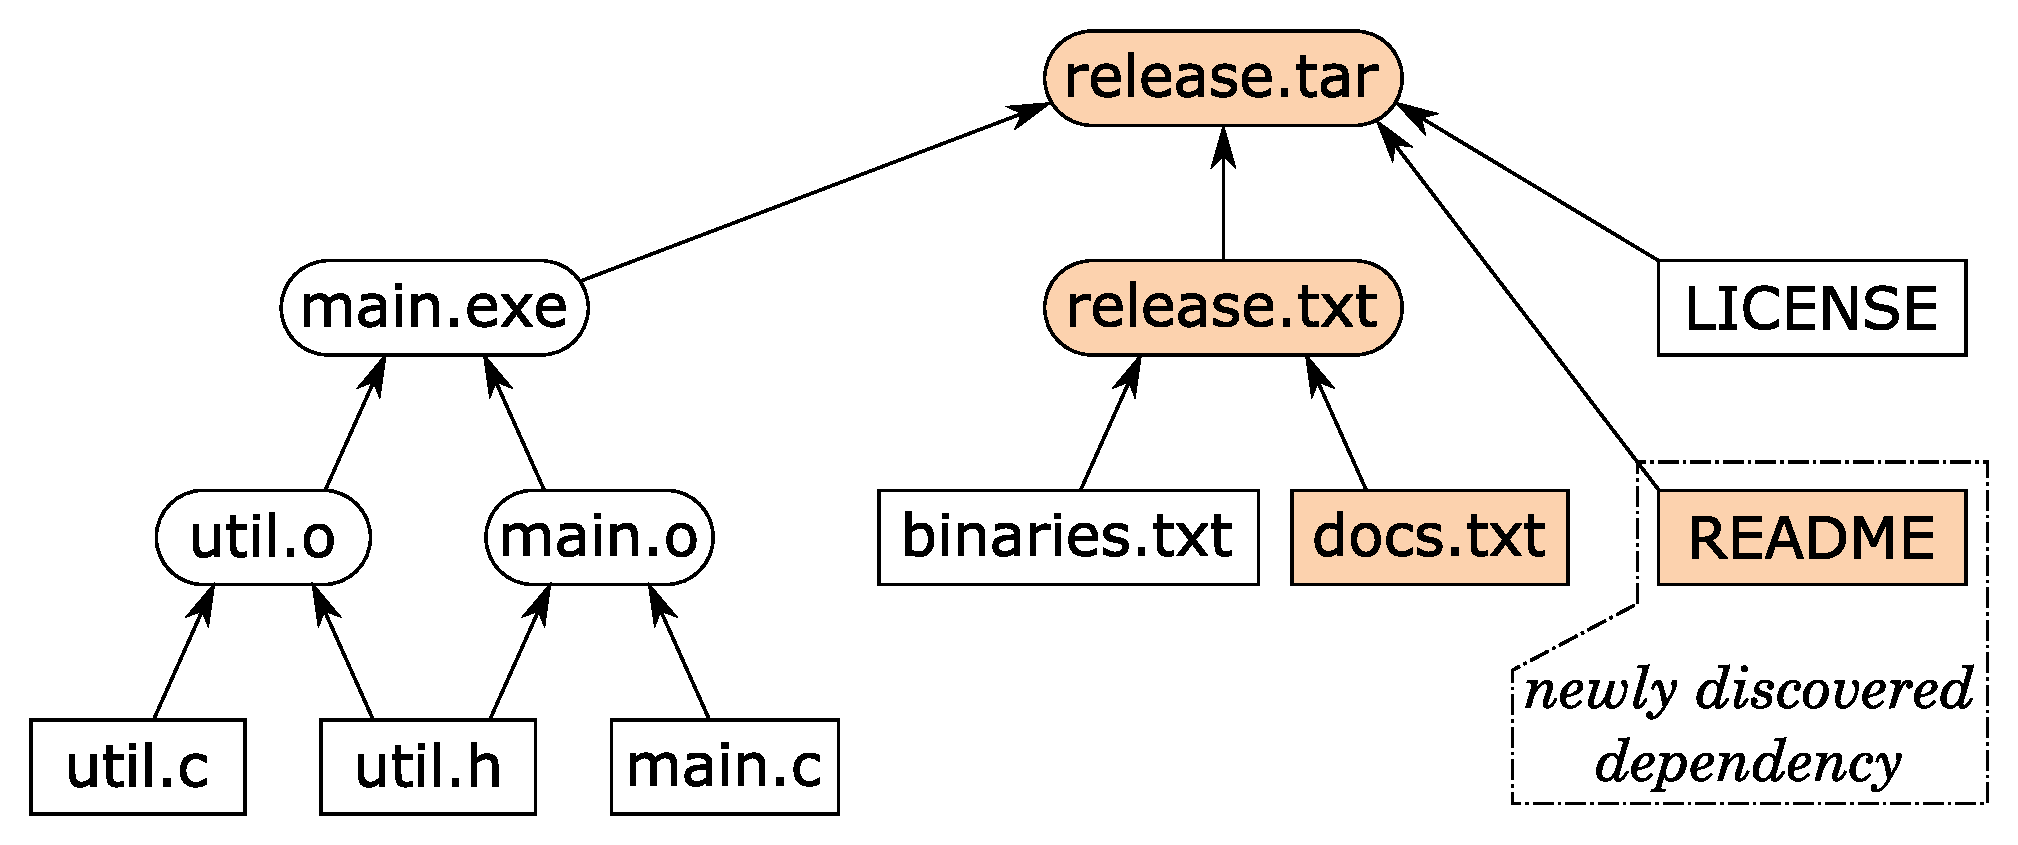
\includegraphics[scale=0.28]{fig/shake-example-rebuild.pdf}}
\caption{Since \cmd{docs.txt} was modified, we rebuild \cmd{release.txt} and
\cmd{release.tar}, discovering a new dependency.}
\end{subfigure}
\vspace{-2mm}
\caption{Dynamic dependencies example: create \cmd{README} and add it to the
list of release documents \cmd{docs.txt}.\label{fig-shake}}
\vspace{-4mm}
\end{figure}

\subsection{\Shake: dynamic dependencies with no remorse}
\label{sec-background-shake}

\Shake was developed to solve the issue of dynamic
dependencies~\cite{mitchell2012shake} without sacrificing
the minimality requirement. Building on the \Make example
from~\S\ref{sec-background-make}, we add the following files whose
dependencies are shown in Fig.~\ref{fig-shake}(a):

\begin{itemize}
    \item \cmd{LICENSE} is an input text file containing the project license.
    \item \cmd{release.txt} is a text file listing all files that should be in the release. This file
    is produced by concatenating input files \cmd{bins.txt} and \cmd{docs.txt},
    which list all binary and documentation files of the project.
    \item \cmd{release.tar} is the release archive built by executing the
    command \cmd{tar} on the release files.
\end{itemize}

The dependencies of \cmd{release.tar} are not known statically: they are
determined by the content of \cmd{release.txt}, which might not even exist
before the build. Makefiles cannot express such dependencies, requiring problematic
workarounds such as \emph{build phases} \cite{hadrian}.
In \Shake we can express the rule for \cmd{release.tar} as:

\begin{minted}[xleftmargin=10pt]{haskell}
"release.tar" %> \_ -> do
    need ["release.txt"]
    files <- lines <$> readFile "release.txt"
    need files
    system "tar" $ ["-cf", "release.tar"] ++ files
\end{minted}

\noindent
We first declare the static dependency on \cmd{release.txt}, then read its
content (a list of files) and depend on each listed file, dynamically. Finally, we specify the
command to produce the resulting archive. Crucially, the archive will only be
rebuilt if one of the dependencies (static or dynamic) has changed. For example,
if we create another documentation file \cmd{README} and add it to
\cmd{docs.txt}, \Shake will appropriately rebuild \cmd{release.txt} and
\cmd{release.tar}, discovering the new dependency, see Fig.~\ref{fig-shake}(b).

\Shake's implementation is different from both \Make and \Excel in two aspects.
First, it uses the dependency graph from the previous build to decide which
files need to be rebuilt. This idea has a long history, going back to
\emph{incremental}~\cite{demers1981incremental},
\emph{adaptive}~\cite{acar2002adaptive}, and
\emph{self-adjusting computations} (see \cite{acar2007selfadjusting} and
\S\ref{sec-related}). Second, instead of aborting and deferring the execution of
tasks whose newly discovered dependencies have not yet been built (as \Excel
does), \Shake \emph{suspends} their execution until the dependencies are brought
up to date. We refer to this task scheduling algorithm as \emph{suspending},
see a concrete implementation in~\S\ref{sec-implementation-shake}.

\begin{figure}
\vspace{-3mm}
\centerline{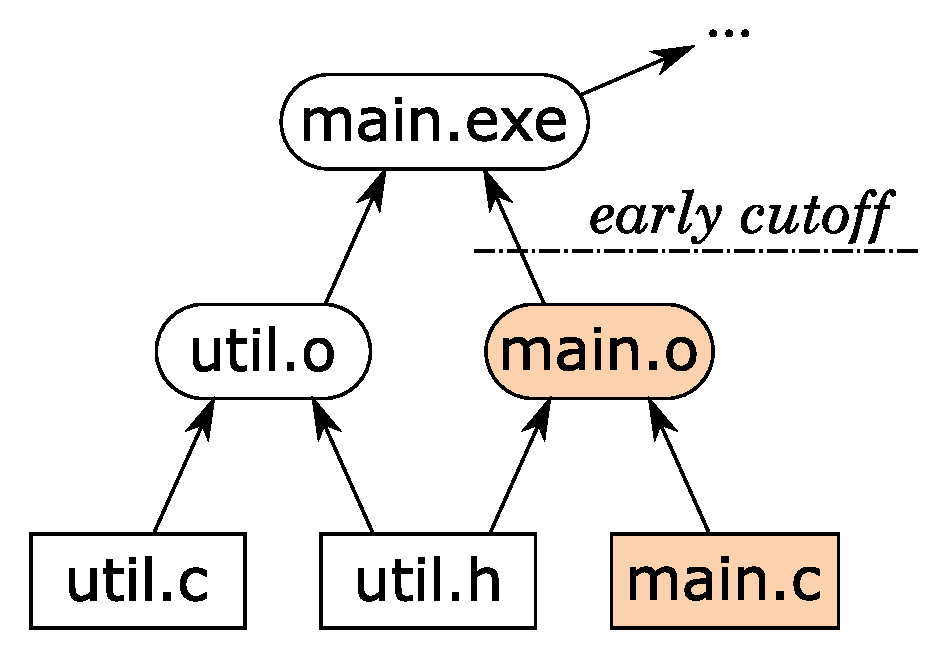
\includegraphics[scale=0.28]{fig/shake-example-cutoff.pdf}}
\vspace{-4mm}
\caption{An early cutoff example: if a comment is added to \cmd{main.c}, the
rebuild is stopped after detecting that \cmd{main.o} is unchanged, since this
indicates that \cmd{main.exe} and its dependents do not need to be
rebuilt.\label{fig-cutoff}}
\vspace{-4mm}
\end{figure}

\Shake also supports the \emph{early cutoff optimisation}. When it
executes a task and the result is unchanged from the previous build, it is
unnecessary to execute the dependent tasks, and hence \Shake can stop a build
earlier, as illustrated in Fig.~\ref{fig-cutoff}. Not all build systems support
early cutoff: \Make and \Excel do not, whereas \Shake and \Bazel (introduced
below) do.

\vspace{-0.5mm}
\subsection{\Bazel: a cloud build system}\label{sec-background-bazel}
\vspace{-0.5mm}

When build systems are used by large teams, different team members often end up
executing exactly the same tasks on their local machines. A \emph{cloud build
system} can speed up builds dramatically by sharing build results
among team members. Furthermore, cloud build systems can support \emph{shallow
builds} that materialise only end build products locally, leaving all
intermediates in the cloud.

Consider an example in Fig.~\ref{fig-bazel}. The user starts by downloading the
sources, whose content hashes are (for simplicity)~1,~2 and~3, and requests to
build \cmd{main.exe}, see Fig.~\ref{fig-bazel}(a,b). By looking up the global
history of all previous builds\footnote{In practice, old entries are regularly
evicted from the cloud storage, as further discussed
in~\S\ref{sec-cloud-aspects}.}, the build system finds that someone has already
compiled these exact sources before and the resulting files \cmd{util.o} and
\cmd{main.o} had hashes 4~and~5, respectively. Similarly, the build system finds
that the hash of the resulting \cmd{main.exe} was 6 and downloads the actual
binary from the cloud storage -- it must be materialised, because it is the end
build product.

In Fig.~\ref{fig-bazel}(c), the user modifies the source file \cmd{util.c},
thereby changing its hash from~1~to~7. The cloud lookup of the new combination
$\{\cmd{util.c}, \cmd{util.h}\}$ fails, which means that nobody has ever
compiled it. The build system must therefore build \cmd{util.o}, materialising
it with the new hash~8. The combination of hashes of \cmd{util.o} and
\cmd{main.o} has not been encountered before either, thus the build system first
downloads \cmd{main.o} from the cloud and then builds \cmd{main.exe} by linking
the two object files. When the build is complete, the results can be uploaded to
the cloud for future reuse by other team members.

\Bazel is one of the first openly-available cloud build systems.
As of writing, it is not possible to express dynamic dependencies in
user-defined build rules; however some of the pre-defined build rules require
dynamic dependencies and the internal build engine can cope with them by using
a \emph{restarting} task scheduler, which is similar to that of \Excel but does
not use the calc chain. \Bazel is not minimal in the sense that it may restart a
task multiple times as new dependencies are discovered and rebuilt, but it
supports the early cutoff optimisation.

To support cloud builds, \Bazel maintains (i) a \emph{content-addressable cache}
that can be used to download a previously built file given the hash of its
content, and (ii) the history of all executed build commands annotated with
observed file hashes. The latter allows the build engine to bypass the execution
of a task, by predicting the hash of the result from the hashes of its
dependencies, and subsequently download the result from the cache. A concrete
implementation is provided in~\S\ref{sec-implementation-cloud}.

\begin{figure}
\vspace{-2mm}
\begin{subfigure}[b]{0.25\linewidth}
\centerline{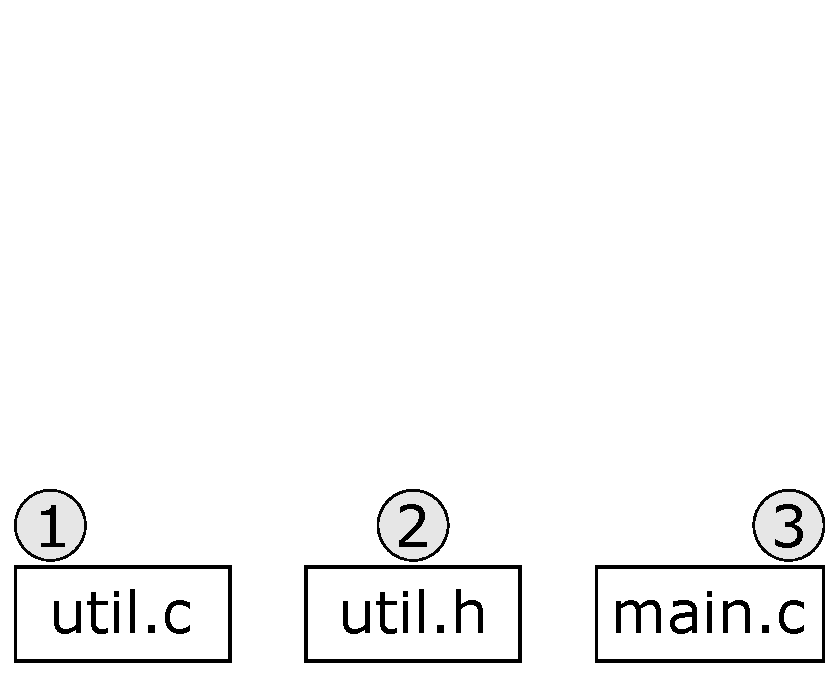
\includegraphics[scale=0.28]{fig/bazel-example-checkout.pdf}}
\vspace{-1mm}
\caption{Download source files}
\end{subfigure}
\begin{subfigure}[b]{0.40\linewidth}
\centerline{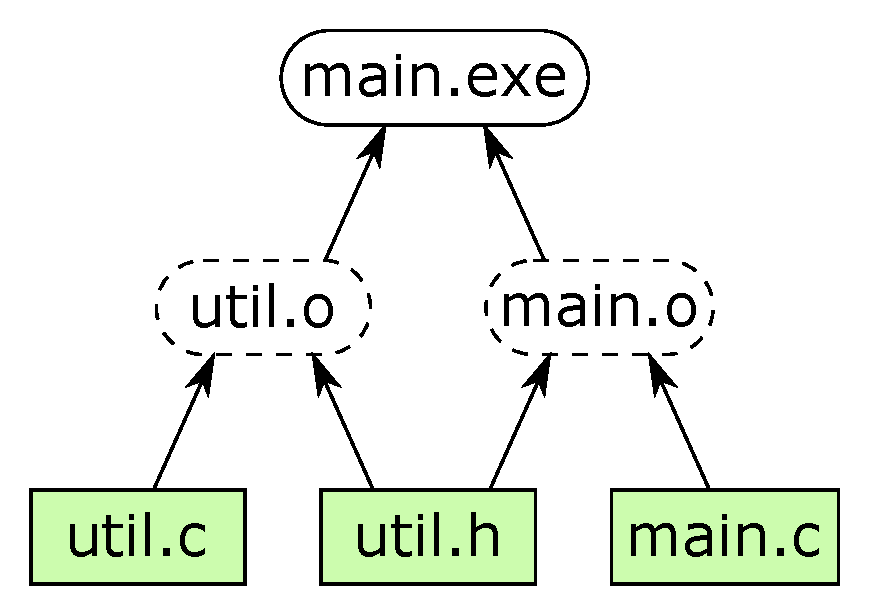
\includegraphics[scale=0.28]{fig/bazel-example-build.pdf}}
\vspace{-1mm}
\caption{Build \cmd{main.exe}}
\end{subfigure}
\begin{subfigure}[b]{0.31\linewidth}
\centerline{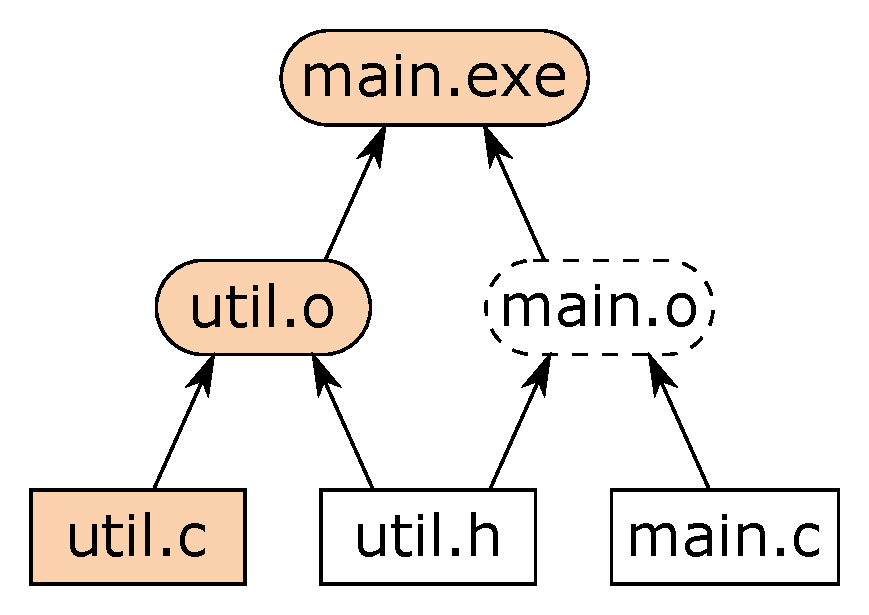
\includegraphics[scale=0.28]{fig/bazel-example-rebuild.pdf}}
\vspace{-1mm}
\caption{Modify \cmd{util.c} and rebuild}
\end{subfigure}
\vspace{-2.5mm}
\caption{A cloud build example: (a)~download sources, (b)~build \cmd{main.exe}
by downloading it from the cloud and skipping intermediate files (only their
hashes are needed), (c)~modify \cmd{util.c} and rebuild \cmd{main.exe}, which
requires building \cmd{util.o} (nobody has compiled \cmd{util.c} before) and
downloading \cmd{main.o} (it is needed for linking \cmd{main.exe}). File hashes
are shown in circles, and non-materialised intermediates in dashed rounded
rectangles.\label{fig-bazel}}
\vspace{-3mm}
\end{figure}

\begin{table}[h]
\vspace{-1mm}
\smaller
\centering
\begin{tabular}{l||l|l||l|c|c|c}
\hline
$\!$Build system$\!$& Persistent build information & Scheduler   & Dependencies    & Minimal & Cutoff & Cloud$\!$\\\hline
$\!$\Make       $\!$& File modification times      & Topological & Static          & Yes     & No     & No   $\!$\\
$\!$\Excel      $\!$& Dirty cells, calc chain      & Restarting  & Dynamic         & No      & No     & No   $\!$\\
$\!$\Shake      $\!$& Previous dependency graph    & Suspending  & Dynamic         & Yes     & Yes    & No   $\!$\\
$\!$\Bazel      $\!$& Cloud cache, command history & Restarting  & Dynamic$^{(*)}$ & No      & Yes    & Yes  $\!$\\\hline
\hline
\end{tabular}
\caption{Build system differences; $^{(*)}$at present, user-defined build rules
cannot have dynamic dependencies.\label{tab-summary}}
\vspace{-8mm}
\end{table}

\vspace{-1.5mm}
\subsection{Summary}\label{sec-background-summary}
\vspace{-0.5mm}

We summarise differences between four discussed build systems in
Table~\ref{tab-summary}. The column \emph{`persistent build information'} refers
to the information that build systems persistently store between builds:
\begin{itemize}
    \item \Make stores file modification times, or rather, it relies on the file
    system to do that.
    \item \Excel stores one dirty bit per cell and the calc chain from the
    previous build.
    \item \Shake stores the dependency graph discovered in the previous build,
    annotated with file content hashes for efficient checking of file changes.
    \item \Bazel stores the content-addressable cache and the history of all
    previous build commands annotated with file hashes. This information is
    shared among all users of the build system.
\end{itemize}

In this paper we elucidate which build system properties are consequences of
specific implementation choices (stored metadata and task scheduling algorithm),
and how one can obtain new build systems with desired properties by recombining
parts of existing implementations. As a compelling example,
in~\S\ref{sec-implementation-cloud} we demonstrate how to combine the advantages
of \Shake and \Bazel.

\section{Build systems, abstractly}\label{sec-compute}

This section presents purely functional abstractions that allow us to express
all the intricacies of build systems discussed in the previous
section~\S\ref{sec-background} and design complex build systems from simple
primitives. Specifically, we present the \emph{compute} and \emph{build}
abstractions, which are described in
Sections~\ref{sec-task} and \ref{sec-general-build} respectively.

\vspace{1mm}
\begin{minted}[xleftmargin=10pt]{haskell}
type Task c k v = @\std{forall}@ f. c f => (k -> f v) -> k -> Maybe (f v)
type Build c i k v = Task c k v -> k -> Store i k v -> Store i k v
\end{minted}
\vspace{1mm}

\hs{Build} corresponds to the algorithm used for bringing a key-value store
\store to a consistent state by recomputing out-of-date values in an
appropriate order. We explain the build type and use it to develop a formal
definition of build systems in~\S\ref{sec-general-build}.
Sections~\S\ref{sec-build} and~\S\ref{sec-implementations} scrutinise the build
abstraction further and provide concrete implementations for several build
systems.

\subsection{Common vocabulary for build systems}
\label{sec-vocabulary}

\begin{figure}
\begin{minted}{haskell}
-- Stores
data Store i k v   -- Abstract
getInfo  :: Store i k v -> i
putInfo  :: Store i k v -> i -> Store i k v
getValue :: Store i k v -> k -> v
putValue :: Hashable v => Store i k v -> k -> v -> Store i k v
getHash  :: Hashable v => Store i k v -> k -> Hash

-- Hashing
hash :: Hashable a => a -> Hash

-- Applicative
(<*>) :: Applicative f => f (a->b) -> f a -> f b  -- Left-associative
(<$>) :: Applicative f => (a->b) -> f a -> f b    -- Left-associative
pure  :: Applicative f => a -> f a

-- State monad
data State s
instance Applicative State
instance Monad       State
evalState :: State s a -> s -> s
getState  :: State s s
\end{minted}
\caption{Signatures of library functions}
\label{fig-lib-funs}
\end{figure}

We start by establishing a common vocabulary for build systems that allows
us to abstract away from specific application domains, such as software
development or spreadsheets.
% We will use this vocabulary throughout the rest of the paper.

A \emph{build system} takes a \emph{task description}, a target \emph{key},
and a \emph{store}, and returns a new store in which the target key is
up to date.  The store is a key/value mapping, togther with
\emph{persistent build state} that is maintained by the build system itself.

In software build systems, keys are typically filenames,
e.g.~\cmd{main.c}, and values are file contents (a C program source
code in this case). In spreadsheets, keys are cell names,
e.g. \cmd{A1}, and values are numbers, text, etc. that are typically
displayed inside cells. In our Haskell code, we will use type
variables \hs{k} and \hs{v} to denote keys and values, respectively.

Some values must be provided by the user as \emph{input}. For example,
\cmd{main.c} can be edited by the user who relies on the build system to
compile it into \cmd{main.o} and subsequently \cmd{main.exe}. End build products,
such as \cmd{main.exe}, are \emph{output} values. All other values (in this case
\cmd{main.o}) are \emph{intermediate}; they are not interesting for the user
but are produced in the process of turning inputs into outputs.

The types of the library functions we use in this paper is
given in Figure~\ref{fig-lib-funs}.
We use a cryptographic \emph{hash function} \hs{hash :: Hashable v =>
v -> Hash} for efficient tracking and sharing of~build results, where
\hs{Hash} is an abstract data type equipped with the equality test.

A \emph{store}, of type \hs{Store i k v}, associates keys to values.
It is convenient to assume that a
store is total function \store, i.e. it contains a value for every possible key.
We therefore also assume that the type of values is capable of encoding values
corresponding to non-existent keys (missing files or empty cells). This, in
particular, suggests that it is possible to \emph{depend on the absence of a
value}, which is a useful feature for build systems. In addition to usual
read and write operations, some stores also support a dedicated \emph{read hash}
operation, which is implemented more efficiently than by reading and hashing the
result. For example, GVFS (Git Virtual File System)~\cite{gvfs} stores file
hashes and downloads file contents only on demand -- an important feature for
cloud build systems.

The store also contains a single persistent value, of type \hs{i}, representing
the persistent state maintained by the build system itself -- its ``memory''.

\subsection{The Task abstraction}\label{sec-task}

Our first key idea is the task-description abstraction:
\begin{minted}[xleftmargin=10pt]{haskell}
type Task c k v = @\std{forall}@ f. c f => (k -> f v) -> k -> Maybe (f v)
\end{minted}
This highly-abstracted type is best introduced through an example.
Consider this Excel spreadsheet (c.f. \S\ref{sec-background-excel}):
\vspace{1mm}
\begin{minted}[xleftmargin=10pt]{bash}
  A1: 10     B1: =A1 + A2
  A2: 20     B2: =B1 * 2
\end{minted}
\vspace{1mm}
Here cell \hs{A1} contains the value \hs{10} while cell \hs{B1} contains
the formula \hs{=A1+A2}.
We can represent the formulae of of this spreadsheet
with the following task description
\vspace{1mm}
\begin{minted}[xleftmargin=10pt]{haskell}
sprsh1 :: Compute Applicative String Integer
sprsh1 fetch "B1" = Just ((+)   <$> fetch "A1" <*> "A2")
sprsh1 fetch "B2" = Just ((* 2) <$> fetch "B1")
sprsh1 _   _      = Nothing
\end{minted}
\vspace{1mm}
Here we instantiate keys \hs{k} with \hs{String}, and values \hs{v} with \hs{Integer}.
(Real spreadsheet cells would contain a wider range of values, of course.)
The task description \hs{sprsh1} embodies all the \emph{formulae} of the spreadsheet,
but not the constant values.  Like every \hs{Task}, \hs{sprsh1} is given
a \hs{fetch} function and a key. It pattern-matches on the key to see if it has
a task description (in the Excel case, a formula)
for it.  If not, it returns \hs{Nothing}, indicating that there is no formula in
that cell.  If there is a formula in the cell, it computes
the value of the formula, using \hs{fetch} to find the value of any keys on
which it depends.

The code to ``compute the value of a formula'' in \hs{sprsh1} looks a bit mysterious
because it takes place in an \hs{Applicative} computation \cite{mcbride2008applicative}
-- the relevant type signatures
are given in Figure~\ref{fig-lib-funs}.  We will return to the need for this
generality in
Section~\ref{sec-deps}\footnote{Readers familiar with \emph{lenses} or \emph{profunctor optics}
might recognise a familiar pattern. We discuss this in~\S\ref{sec-related-optics}.}.

For now, we content ourselves with observing that a task description,
of type \hs{Task c k v}, is completely isolated from the world of
compilers, calculation chains, file systems, caches, and all other
complexities of real build systems.  It just computes a single output, in
a side-effect-free way, using a call-back (\hs{fetch}) to obtain the values
of its dependencies.

\subsection{The Build abstraction}\label{sec-general-build}

Next comes our second key abstraction: a build system:
\vspace{1mm}
\begin{minted}[xleftmargin=10pt]{haskell}
type Build c i k v = Task c k v -> k -> Store i k v -> Store i k v
\end{minted}
\vspace{1mm}
The signature is very straightforward.  Given a task description, a target key,
and a store, the build system returns a new store in which the value of the
target key is up-to-date.  (What exactly does ``up to date'' mean?  We answer
that precisely in \S\ref{sec-build-correctness}.

\emph{SLPJ: is this right?}
\vspace{1mm}
\begin{minted}[xleftmargin=10pt]{haskell}
dumbBuild :: Build Monad () k v
dumbBuild task k store = execState (go k) store
  where
    go :: k -> State s v
    go k = case (task go k) of
             Nothing  -> do { s <- getState; return (getValue s k) }
             Just act -> do { v <- act; updState (\s -> putStore s k v); return v }
\end{minted}
\vspace{1mm}
\emph{SLPJ: explain}

\subsection{Correctness of a build system} \label{sec-build-correctness}

We can now say what it means for a build system to be \emph{correct}, something
that is seldom stated formally:

\definition[Correctness]{Suppose \hs{build :: Build c i k v} is a build system,
\hs{task :: Task c k v} describes an acyclic collection of build tasks, \hs{key} is an output
key, \hs{store} be a store.
Then the \hs{result}ing store \hs{result = build compute key store}
is~\emph{correct} if there exists a store \hs{ideal}, such that

\begin{itemize}
    \item The \hs{ideal} store is \emph{consistent} with \hs{task}, i.e.
    for all possible non-input keys \hs{k}, the result of executing the
    \hs{compute} matches the value in the \hs{ideal} store:
    \[
    \hs{execute}~\hs{ideal}~\hs{k}~\hs{==}~\hs{Just}~\hs{(}\hs{ideal}~\hs{k)}.
    \]
    \item The \hs{result} and \hs{ideal} agree on the output \hs{key}, i.e.
    \hs{result}~\hs{key}~\hs{==}~\hs{ideal}~\hs{key}. In other words, we require
    that the output \hs{key} has the correct value, but do not impose any
    restrictions on intermediate keys, therefore permitting shallow cloud builds.
    \item The \hs{store}, \hs{ideal} and \hs{result} all agree on the inputs
    that belong to the transitive closure of \hs{key}'s dependencies. This means
    that (i) no inputs were corrupted during the build, and (ii)~the \hs{ideal}
    store has constraints not only on the output, but also on the inputs.
\end{itemize}
}
\label{def-correct}


\subsection{Computing dependencies}

The \hs{Compute} type and the example above might seem mysterious. Why insist on
\hs{Compute} to be polymorphic in \hs{f}? Why choose the \hs{Applicative}
constraint?

The answer to both questions is that we can statically analyse an applicative
compute and extract all dependencies of a key using the following function:

\vspace{1mm}
\begin{minted}[xleftmargin=10pt]{haskell}
import Data.Functor.Const
\end{minted}
\vspace{0.5mm}
\begin{minted}[xleftmargin=10pt]{haskell}
dependencies :: Compute Applicative k v -> k -> [k]
dependencies compute = maybe [@@] getConst . compute (\k -> Const [k])
\end{minted}
\vspace{1mm}

\noindent
We can use this function to extract dependencies of \hs{add}, as shown in the
following GHCi session:

\vspace{1mm}
\begin{minted}[xleftmargin=10pt]{haskell}
@\ghci@ dependencies add "A1"
[@@]
\end{minted}
\begin{minted}[xleftmargin=10pt]{haskell}
@\ghci@ dependencies add "B1"
["A1", "A2"]
\end{minted}
\vspace{1mm}

\noindent
It is important to note that we extract the dependencies without providing any
values to the compute. This guarantees that no actual computation is performed
during the analysis -- we cannot execute the function \hs{(+)} if we have no
values for it! Static analysis of applicative computations is not new and has
been used to similar effect before, e.g. see~\cite{free-applicatives}.

To understand how \hs{dependencies} works, let us examine its type more closely,
expanding the type synonym \hs{Compute}:

\vspace{1mm}
\begin{minted}[xleftmargin=10pt]{haskell}
(@\std{forall}@ f. Applicative f => (k -> f v) -> k -> Maybe (f v)) -> k -> [k]
\end{minted}
\vspace{1mm}

\noindent
Since the first argument is polymorphic in \hs{f}, we can choose any \hs{f} that
satisfies the \hs{Applicative} constraint. A good choice in this case is the
applicative functor \hs{Const}:

\vspace{1mm}
\begin{minted}[xleftmargin=10pt]{haskell}
newtype Const m a = Const { getConst :: m }
\end{minted}
\vspace{0.5mm}
\begin{minted}[xleftmargin=10pt]{haskell}
instance Functor (Const m) where
    fmap _ (Const m) = Const m
\end{minted}
\vspace{0.5mm}
\begin{minted}[xleftmargin=10pt]{haskell}
instance Monoid m => Applicative (Const m) where
    pure _              = Const mempty
    Const x <*> Const y = Const (x <> y)
\end{minted}
\vspace{1mm}

\noindent
A value of type \hs{Const}~\hs{[}\hs{k]}~\hs{v} contains no values \hs{v} but
allows us to record all invocations of the custom \hs{fetch} function that we
feed to the given compute: \hs{fetch k = Const [k]}. The compute returns a
value of type \hs{Maybe}~\hs{(Const}~\hs{[}\hs{k]}~\hs{v)} that can be
unwrapped using \hs{maybe [@@] getConst}, i.e. returning the empty list of
dependencies in case of an input.

We can also \hs{execute} a compute on a given store. This relies on a similar
transformation, now based on the \hs{Identity} monad (see
Appendix~\S\ref{sec-appendix-transformers} for the implementation of
\hs{Identity}):

\vspace{1mm}
\begin{minted}[xleftmargin=10pt]{haskell}
import Data.Functor.Identity
\end{minted}
\vspace{0.5mm}
\begin{minted}[xleftmargin=10pt]{haskell}
execute :: Compute Monad k v -> (k -> v) -> k -> Maybe v
execute compute store = fmap runIdentity . compute (pure . store)
\end{minted}
\vspace{1mm}

\noindent
Note that \hs{execute} can accept both an applicative as well as a \emph{monadic
compute} introduced in~\S\ref{sec-compute-monad}. Below we run \hs{execute} on
the above \hs{add} example. Note that \hs{execute} returns \hs{Nothing} for
inputs.

\vspace{1mm}
\begin{minted}[xleftmargin=10pt]{haskell}
@\ghci@ store key = if key == "A1" then 10 else 20
@\ghci@ execute add store "A1"
Nothing
\end{minted}
\begin{minted}[xleftmargin=10pt]{haskell}
@\ghci@ execute add store "B1"
Just 30
\end{minted}

\subsection{Monadic compute}\label{sec-compute-monad}

As discussed in~\S\ref{sec-background}, some build tasks have dynamic
dependencies, which are determined by values of intermediate computations. In
our framework, such build tasks correspond to \emph{monadic compute}, i.e.
the type \hs{Compute}~\hs{Monad}~\hs{k}~\hs{v}. Recall the following spreadsheet
example:

\vspace{1mm}
\begin{minted}[xleftmargin=10pt]{bash}
A1 = 10
A2 = 20
B1 = IF(C1=1,A1,A2)
C1 = 1
\end{minted}
\vspace{1mm}

\noindent
The task corresponding to the cell \cmd{B1} statically depends on \cmd{C1} and
dynamically depends on either \cmd{A1} or \cmd{A2}. We can express this using
our compute abstraction as follows\footnote{The spreadsheet example that uses
the \hs{INDIRECT} function can be expressed very similarly: simply replace the
last line of the \hs{select} function with \hs{fetch ("A" ++ show c1)}.}:

\vspace{1mm}
\begin{minted}[xleftmargin=10pt]{haskell}
select :: Compute Monad String Integer
select fetch key | key /= "B1" = Nothing
                 | otherwise   = Just $ do
                     c1 <- fetch "C1"
                     if c1 == 1 then fetch "A1" else fetch "A2"
\end{minted}
\vspace{1mm}

We cannot statically analyse \hs{select} using the function \hs{dependencies}
from the previous section, but we can still \hs{execute} it on a given store:

\vspace{1mm}
\begin{minted}[xleftmargin=10pt]{haskell}
@\ghci@ store key = if key == "A1" then 10 else 20
@\ghci@ execute select store "B1"
Just 20
\end{minted}
\vspace{1mm}

\noindent
In the example above $\cmd{C1} \neq 1$, hence the \hs{else} branch is taken.
To extract the dependencies of \hs{select} we introduce the function \hs{track}:
a combination of \hs{execute} and \hs{dependencies} that takes the store~\store
as input and computes both the resulting value and the list of its dependencies:

\vspace{1mm}
\begin{minted}[xleftmargin=10pt]{haskell}
import Control.Monad.Writer
\end{minted}
\vspace{0.5mm}
\begin{minted}[xleftmargin=10pt]{haskell}
track :: Compute Monad k v -> (k -> v) -> k -> Maybe (v, [k])
track compute store = fmap runWriter . compute (\k -> writer (store k, [k]))
\end{minted}
\vspace{1mm}

\noindent
The implementation uses the \hs{Writer} monad (\S\ref{sec-appendix-transformers}):
we feed \hs{fetch k = writer (store k, [k])} to the compute, which in addition
to fetching a value from the store, tracks the corresponding key. We can
\hs{track} both applicative and monadic compute:

\vspace{1mm}
\begin{minted}[xleftmargin=10pt]{haskell}
@\ghci@ store key = if key == "A1" then 10 else 20
@\ghci@ track add store "B1"
Just (30,["A1","A2"])
\end{minted}
\vspace{1mm}
\begin{minted}[xleftmargin=10pt]{haskell}
@\ghci@ track select store "B1"
Just (20,["C1","A2"])
\end{minted}
\vspace{1mm}
\begin{minted}[xleftmargin=10pt]{haskell}
@\ghci@ store' key = if key == "A1" then 10 else 1
@\ghci@ track select store' "B1"
Just (10,["C1","A1"])
\end{minted}
\vspace{1mm}

\noindent
As expected, the dependencies of \hs{select} are determined by the contents of
the store.

% \subsection{Recognising an applicative compute wearing a monadic hat}

% Although dynamic dependencies are very useful, they typically represent only a
% small fraction of all dependencies. One can exploit this in a build system by
% recognising applicative computations even though they have the type
% \hs{Compute}~\hs{Monad} and treating them specially.

% Consider the following data type.

% \subsection{Free build structures}\label{sec-free-build}

% \begin{minted}{haskell}
% data Depend k v r = Depend [k] ([v] -> r)

% data Depends k v r = Depends [k] ([v] -> Depends k v r)
%                    | Done r
% \end{minted}



\section{Build Systems \`a la Carte}\label{sec-build}

The focus of this paper is on a variety of implementations of \hs{Build}, given
a \emph{client-supplied} implementation of \hs{Task}. That is, we are going to take
\hs{Task} as given from now on, and explore variants of \hs{Build}: first
abstractly (in this section) and then concretely in~\S\ref{sec-implementations}.

\todo{SLPJ}{What does this para add?}
Let \hs{result}~\hs{=}~\hs{build}~\hs{task}~\hs{key}~\hs{store}. The build
system \hs{build} is responsible for ensuring that \hs{key} and its dependencies
are up-to-date in \hs{result} starting from \hs{store} (\S\ref{sec-build-correctness}). As part of that work,
\hs{build} \emph{may} store auxiliary information \hs{info} of type \hs{i} in
the \hs{store}, which will be provided to future calls of \hs{build}.

\todo{SLPJ}{What does this para add?}
All the build systems we define are polymorphic in both \hs{k} and \hs{v}
(perhaps adding constraints to them), and have specific instantiations of \hs{c}
and \hs{i}. As an example, recall that the \hs{busy} build system defined
in~\S\ref{sec-general-build}, has \hs{c}~\hs{=}~\hs{Monad}, i.e. it supports
monadic tasks, and \hs{i = ()}, i.e. it does not store any build information.

According to the definition of minimality~\ref{def-minimal}, a minimal build
system must \textbf{rebuild only out-of-date keys} and at most once. The only
way to achieve the ``at most once'' requirement is to \textbf{build all keys in
the order that respects their dependencies}.

We have emphasised two different phrases above, and tackle each aspect separately.

\subsection{Respecting the dependency order}
\label{sec-dependency-orderings}

The build systems overview (\S\ref{sec-background-summary}) highlighted three
distinct approaches to respecting the dependency order. This subsection explores
their properties and possible implementations.

\subsubsection{Topological}

The topological approach pre-computes a linear order, which when followed, ensures
the \hs{build} is correct regardless of the initial \hs{store}. Given a function
from a key to its dependencies, and the output \hs{key}, you can compute the
linear order by first taking the transitive closure of \hs{key}'s dependencies,
and then computing its topological sort. However, as we have seen
in~\S\ref{sec-deps}, we can only extract dependencies from an applicative task,
which requires the build system to choose \hs{c}~\hs{=}~\hs{Applicative}, ruling
out dynamic dependencies.

\subsubsection{Reordering}

The topological approach has two downsides: it is limited to \hs{Applicative}
build systems and requires a fresh topological sort each time.  So, while the
actions themselves may be incremental (i.e. unnecessary tasks will not be performed),
the pre-processing is not. We may try to incrementalise the topological sort by
storing the topological order between build runs and assume it to
be correct, but if the build determines it is wrong, fix it up.

This requires a way to abort tasks that have failed due to out-of-date
dependencies. It is also not minimal in the sense that a task may start, do some
meaningful work, then abort. However, in the case of an \hs{Applicative} system,
that work is zero.

\subsubsection{Recursive}

An alternative approach, utilised by the \hs{busy} build system
(\S\ref{sec-general-build}) is to simply build dependencies when they are
requested. By combining that with a transient log of which keys have already
been built, you can obtain a minimal build system.

This requires a way to suspend a running task, which can be done with cheap
green threads and blocking (the original approach of \Shake) or with a
continuation-passing style (what \Shake does now). An alternative approach to
suspending a task is to abort it and restart it again later, at the cost
of doing additional work.

\subsection{Determining out-of-date keys} \label{sec-out-of-date}

The second aspect, determining what to rebuild, can be addressed in one of three
fundamental ways, with a number of tweaks and variations within them.

\subsubsection{A dirty bit}\label{sec-dirty-bit}

The idea of a dirty bit is to have one piece of persistent
information per key, saying whether the key is
\emph{dirty} or \emph{clean}. After a build, all bits are set to clean. When the
next build starts anything that changed between the two states is marked
dirty.
% ; and by marking additional things dirty/clean the build system can track
% what needs to rebuild.
When reaching a key, if it and all its dependencies are
clean, the key does not need recomputing.

\Excel models the dirty bit approach most directly, having an actual dirty bit
associated with each cell, marking the cell it (and its dependencies) dirty
if the user modifies it.
When rebuilding,
if a cell only depends on clean cells it is skipped, otherwise it is rebuilt and
marked dirty itself.
\todo{SLPJ}{What does ``marked dirty itself'' mean?}

% AM: I didn't understand this bit, so commented it out.
% The only wrinkle in this scheme is that \Excel supports
% monadic tasks, and does not separately record the rebuilt, so it has
% to approximate in this case.

\Make uses file modification times, and compares files to their
dependencies, which can be thought of as a dirty bit which is set when
a file is newer than its dependencies. The interesting property of
this dirty bit is that it is not under control of \Make; rather it is
existing file-system information that is repurposed. In particular,
rebuilding a file automatically clears its dirty bit, and
automatically sets the dirty bit of the nodes depending on it. One
thing \Make does require is that file timestamps only go forward in
time -- something that can be violated by backup software.

With a dirty bit it is possible to achieve minimality. To achieve early cutoff
(\S\ref{sec-background-shake}) it would be important to not set the dirty bit
after a computation that did not change the value. \Excel could model this
approach, but does not. In contrast, \Make cannot model early cutoff -- to do so
it would have to mark the node clean (so it didn't rebuild in the next run) and
at the same time not mark the things it depends on dirty -- an impossible task
with only the ability to update to the latest modification time.

\subsubsection{Verifying traces}\label{sec-verifying-traces}

An alternative way to determine if a key is dirty is to record what state the
values/hashes of dependencies were used at last time, and if something has
changed, the key is dirty and must be recomputed -- in essence a \emph{trace}
which we can use to \textit{verify} existing values. We can describe a trace as:

\todo{AM/NM}{Change from \hs{[Trace k v]} to \hs{Map k (Trave k v)} or something
similar, so that it's obvious we have one trace per key .}

\begin{minted}{haskell}
data Trace k v = Trace
    { key          :: k
    , dependencies :: [(k, Hash)]
    , result       :: Hash }
\end{minted}

We assume that \hs{Hash} is a small constant size, constructed from hashing the
underlying \hs{v} rather than storing it directly. Checking a trace requires
ensuring all the dependencies are up-to-date (using whatever ordering strategy
as per \S\ref{sec-dependency-orderings}), then comparing if the dependencies are
same as the current value and that the result is the same. After computing a
fresh value we add its \hs{Trace} to the list. Therefore the information stored
by a build system that verifies traces is \hs{[Trace k v]}.

\subsubsection{Constructive traces}\label{sec-constructive-traces}

A verifying trace allows us to mark a key dirty and rebuild it. Extending that information we can store a \textit{constructive} trace which is the trace plus the actual result. Once we are storing the complete result it makes sense to record many constructive traces per key, and to share them with other users, providing cloud-build functionality. We can represent that as:

\todo{AM/NM}{Traces -- why the indirection (first get the hash, then look it up)?
Can we drop it? Can we switch to a more efficient/explicit data structure than a list?}

\begin{minted}{haskell}
data Traces k v = Traces
    { traces :: [Trace k v]
    , cache  :: Map Hash v }
\end{minted}

We have a list of traces, plus a \hs{Map} from the hash to the actual contents. Checking a trace is the same as before, but if the result is the only thing that is different we can simply retrieve a fresh result from \hs{cache} \textit{without} recomputing it.

For both verifying and constructive choices it is possible to choose smarter data structures than simply a list of \hs{Trace}, which we discuss in \S\ref{sec-smart-traces}.

\todo{AM}{AM: I would also like to see actual \hs{verify} and \hs{construct} functions.

NM: It actually gets a bit more confusing than that - since you end up needing to pass functions to get yourself, your dependencies etc. Unclear there is a win. The functions would occur in the next section anyway.

AM: Now, after we've switched to \hs{Store i k v} it might work better?}

\subsection{Summary} \label{sec-design-space}

\todo{AM/NM/SLPJ}{Add a decription for the table.}

\begin{table}[h]
\smaller
\centering
\begin{tabular}{l||c|c|c}
\hline
Property           & Topological & Reordering & Recursive    \\\hline
\hline
Dirty bit          & \Make                   & \Excel                   & \Shake without early cutoff \\\hline
Verifying trace    & \Make with early cutoff & \Excel with early cutoff & \Shake                      \\\hline
Constructive trace & \Bazel                  & Cloud \Excel             & Cloud \Shake                \\\hline
\end{tabular}
\vspace{0.5mm}
\caption{Build systems \`a la carte.\label{tab-build-systems}}
\end{table}

\section{Build systems, concretely}\label{sec-implementations}

In the previous sections we discussed the types of build systems, and how they
can be broken down into two main components: a scheduler and a rebuilder.
In this section we make this abstract distinction concrete, by
implementing a number of build systems as a composition of a scheduler
and a rebuilder.  Our design is expressed by these types (Fig.~\ref{fig-types}):

\vspace{0.5mm}
\begin{minted}[xleftmargin=10pt]{haskell}
type Scheduler c i ir k v = Rebuilder c ir k v -> Build c i k v
type Rebuilder c   ir k v = k -> v -> Task c k v -> Task (MonadState ir) k v
\end{minted}
\vspace{0.5mm}

\noindent
A \hs{Scheduler} is a function that takes a \hs{Rebuilder} and uses
it to construct a \hs{Build} system, by choosing which keys to rebuild in which
order. The \hs{Rebuilder} makes use of the persistent build information
\hs{ir}, while the scheduler might augment that with further persistent
information of its own, yielding \hs{i}.

A \hs{Rebuilder} takes three arguments: a key, its current value, and a
\hs{Task} that can (re)compute the value of the key if necessary. It uses the
persistent build information \hs{ir} (carried by the state monad) to decide
whether to rebuild the value. If doing so is unnecessary, it returns the current
value; otherwise it runs the supplied \hs{Task} to rebuild it. In both cases it
can choose to update the persistent build information \hs{ir} to reflect what
happened. So a \hs{Rebuilder} wraps a \hs{Task}~\hs{c}~\hs{k}~\hs{v}, which
unconditionally rebuilds the key, to make a
\hs{Task}~\hs{(MonadState}~\hs{ir)}~\hs{k}~\hs{v}, which rebuilds the key only
if necessary, and does the necessary book-keeping. Note that the resulting
\hs{Task} is always monadic; static dependency analysis can be performed on the
original \hs{Task}~\hs{Applicative} if needed.

The scheduler calls the rebuilder, but passes it a \hs{fetch} function
that the latter calls when it needs the value of a dependent key.  This
callback returns control to the scheduler, which may in turn call the
rebuilder to bring the dependent key up to date, and so on.

\begin{figure}
\begin{minted}[fontsize=\small]{haskell}
-- Make build system; stores current time and file modification times
type Time       = Integer
type MakeInfo k = (Time, Map k Time)
\end{minted}
\vspace{0mm}
\begin{minted}[fontsize=\small]{haskell}
make :: Ord k => Build Applicative (MakeInfo k) k v
make = topological modTimeRebuilder
\end{minted}
\vspace{0mm}
\begin{minted}[fontsize=\small]{haskell}
-- A task rebuilder based on file modification times
modTimeRebuilder :: Ord k => Rebuilder Applicative (MakeInfo k) k v
modTimeRebuilder key value task = Task $ \fetch -> do
    (now, modTimes) <- get
    let dirty = case Map.lookup key modTimes of
            Nothing -> True
            time -> any (\d -> Map.lookup d modTimes > time) (dependencies task)
    if not dirty then return value else do
        put (now + 1, Map.insert key now modTimes)
        run task fetch
\end{minted}
\vspace{0mm}
\begin{minted}[fontsize=\small]{haskell}
-- A topological task scheduler
topological :: Ord k => Scheduler Applicative i i k v
topological rebuilder tasks target = execState $ mapM_ build order
  where
    build :: k -> State (Store i k v) ()
    build key = case tasks key of
        Nothing -> return ()
        Just task -> do
            store <- get
            let value = getValue key store
                newTask :: Task (MonadState i) k v
                newTask = rebuilder key value task
                fetch :: k -> State i v
                fetch k = return (getValue k store)
            newValue <- liftStore (run newTask fetch)
            modify $ putValue key newValue
    order = topSort (graph dep target)
    dep k = case tasks k of { Nothing -> []; Just task -> dependencies task }
\end{minted}
\vspace{0mm}
\begin{minted}[fontsize=\small]{haskell}
-- Standard graph algorithms (implementation omitted)
reachable :: Ord k => (k -> [k]) -> k -> Graph k
topSort   :: Ord k => Graph k -> [k] -- Throws error on a cyclic graph
\end{minted}
\vspace{0mm}
\begin{minted}[fontsize=\small]{haskell}
-- Expand the scope of visibility of a stateful computation
liftStore :: State i a -> State (Store i k v) a
liftStore x = do
    (a, newInfo) <- gets (runState x . getInfo)
    modify (putInfo newInfo)
    return a
\end{minted}
\vspace{-3mm}
\caption{An implementation of \Make using our framework.}\label{fig-make-implementation}
\vspace{-5mm}
\end{figure}

These two abstractions are the key to modularity: \emph{we can combine any
scheduler with any rebuilder, and obtain a correct build system}.
In this section we will write a scheduler for each column of
Table~\ref{tab-build-systems}, and a rebuilder for each row; then combine them
to obtain the build systems in the table's body.

\subsection{\Make}\label{sec-implementation-make}

An implementation of \Make using our framework is shown in
Fig.~\ref{fig-make-implementation}. As promised, its definition
is just the application of a \hs{Scheduler}, \hs{topological},
to a \hs{Rebuilder}, \hs{modTimeRebuilder}.
We discuss each component in turn, starting with the rebuilder.

The \hs{modTimeRebuilder} uses the pair
\hs{MakeInfo}~\hs{k}~\hs{=}~\hs{(@@now,}~\hs{modTimes)} as persistent
build information, carried by a state monad. This \hs{MakeInfo} comprises
the \emph{current time} \hs{now}~\hs{::}~\hs{Time} and the map
\hs{modTimes}~\hs{::}~\hs{Map}~\hs{k}~\hs{Time} of \emph{file modification
times}. We assume that the external system, which invokes the build system,
updates \hs{MakeInfo} reflecting any file changes between successive builds.

The rebuilder receives three arguments: a \hs{key}, its current \hs{value}, and
the applicative \hs{task} that can be used to rebuild the \hs{key} if necessary.
The rebuilder first decides if the \hs{key} is \hs{dirty} by consulting
\hs{modTimes}: if the \hs{key} is not found, that must mean it has never been
built before; otherwise \hs{modTimeRebuilder} can see if any of the \hs{task}'s
dependencies (computed by \hs{dependencies}) are out of date. If the \hs{key} is
\hs{dirty}, we use \hs{run}~\hs{task} to rebuild it, and update the state with
the new modification time of the \hs{key}\footnote{The real \Make
relies on the file system to track file modification times, but we prefer
to make it explicit here.}; otherwise we can just return the current \hs{value}.

\Make's scheduler, \hs{topological}, processes keys in a linear \hs{order} based
on a topological sort of the statically known dependency graph
(see~\S\ref{sec-parallelism} for parallel \Make). Our definition in
Fig.~\ref{fig-make-implementation} is polymorphic with respect to the type of
build information \hs{i} and is therefore compatible with any applicative
\hs{rebuilder}. The scheduler calls the supplied \hs{rebuilder} on every
\hs{key} in the \hs{order}, and runs the obtained \hs{newTask} to compute the
\hs{newValue}. Note that \hs{newTask} has access only to the \hs{i} part of the
\hs{Store}~\hs{i}~\hs{k}~\hs{v}, but the rest of the \hs{do} block runs in the
\hs{State}~\hs{(@@Store}~\hs{i}~\hs{k}~\hs{v)} monad; we use the (unremarkable)
helper function \hs{liftStore} to fix the mismatch. The \hs{newTask} finds
values of the \hs{key}'s dependencies via the \hs{fetch} callback, which is
defined to directly read the \hs{store}.

The pre-processing stage uses the function \hs{dependencies}, defined
in~\S\ref{sec-deps}, to extract static dependencies from the provided
applicative \hs{task}. We compute the linear processing \hs{order} by
constructing the graph of keys \hs{reachable} from the \hs{target} via
dependencies, and performing the topological sort of the result. We omit
implementation of textbook graph algorithms \hs{reachable} and \hs{topSort},
e.g. see~\cite{cormen2001introduction}.

Note that the function \hs{dependencies} can only be applied to applicative
tasks, which restricts \Make to static dependencies, as reflected in the
type~\hs{Build}~\hs{Applicative}. Moreover, any other build system that uses
the \hs{topological} scheduler will also inherit the same restriction.

\subsection{\Excel}\label{sec-implementation-excel}

Our model of \Excel uses the \hs{restarting} scheduler and the
\hs{dirtyBitRebuilder}, see Fig.~\ref{fig-excel-implementation}. The persistent
build information \hs{ExcelInfo}~\hs{k} is a pair: (i) a map
\hs{k}~\hs{->}~\hs{Bool} associating a dirty bit with every key, and (ii) a
calc chain of type \hs{[@@k]} recorded in the previous build
(\S\ref{sec-background-excel}).

The external system, which invokes \Excel's build engine, is required
to provide a transitively closed set of dirty bits. That is, if a
cell is changed, its dirty bit is set, as well as the dirty bit of any other
cell whose value might perhaps change as a result. It is OK to mark too many
cells as dirty; but not OK to mark too few.

The \hs{dirtyBitRebuilder} is very simple: if the \hs{key}'s dirty bit is set,
we \hs{run} the \hs{task} to rebuild the \hs{key}; otherwise we return the
current \hs{value} as is.
Because the dirty cells are transitively closed,
unlike \Make's \hs{modTimeRebuilder}, the \hs{dirtyBitRebuilder} does
not need to modify \hs{i} to trigger rebuilds of dependent keys.

\begin{figure}
\begin{minted}[fontsize=\small]{haskell}
-- Excel build system; stores a dirty bit per key and calc chain
type Chain k = [k]
type ExcelInfo k = (k -> Bool, Chain k)
\end{minted}
\vspace{1mm}
\begin{minted}[fontsize=\small]{haskell}
excel :: Ord k => Build Monad (ExcelInfo k) k v
excel = restarting dirtyBitRebuilder
\end{minted}
\vspace{1mm}
\begin{minted}[fontsize=\small]{haskell}
-- A task rebuilder based on dirty bits
dirtyBitRebuilder :: Rebuilder Monad (k -> Bool) k v
dirtyBitRebuilder key value task = Task $ \fetch -> do
    isDirty <- get
    if isDirty key then run task fetch else return value
\end{minted}
\vspace{1mm}
\begin{minted}[fontsize=\small]{haskell}
-- A restarting task scheduler
restarting :: Ord k => Scheduler Monad (ir, Chain k) ir k v
restarting rebuilder tasks target = execState $ do
    chain    <- gets (snd . getInfo)
    newChain <- liftChain $ go Set.empty $ chain ++ [target | target `notElem` chain]
    modify $ mapInfo $ \(ir, _) -> (ir, newChain)
  where
    go :: Set k -> Chain k -> State (Store ir k v) (Chain k)
    go _    []       = return []
    go done (key:keys) = case tasks key of
        Nothing -> (key :) <$> go (Set.insert key done) keys
        Just task -> do
            store <- get
            let newTask :: Task (MonadState ir) k (Either k v)
                newTask = try $ rebuilder key (getValue key store) task
                fetch :: k -> State ir (Either k v)
                fetch k | k `Set.member` done = return $ Right (getValue k store)
                        | otherwise           = return $ Left k
            result <- liftStore (run newTask fetch) -- liftStore is defined in Fig. 7
            case result of
                Left dep -> go done $ dep : filter (/= dep) keys ++ [key]
                Right newValue -> do modify $ putValue key newValue
                                     (key :) <$> go (Set.insert key done) keys
\end{minted}
\vspace{1mm}
\begin{minted}[fontsize=\small]{haskell}
-- Convert a total task into a task that accepts a partial fetch callback
try :: Task (MonadState i) k v -> Task (MonadState i) k (Either e v)
try task = Task $ \fetch -> runExceptT $ run task (ExceptT . fetch)
\end{minted}
\vspace{1mm}
\begin{minted}[fontsize=\small]{haskell}
-- Expand the scope of visibility of a stateful computation (implementation omitted)
liftChain :: State (Store ir k v) a -> State (Store (ir, Chain [k]) k v) a
\end{minted}
\vspace{-2.5mm}
\caption{An implementation of \Excel using our framework.}\label{fig-excel-implementation}
\vspace{-2.5mm}
\end{figure}

\Excel's \hs{restarting} scheduler processes keys in the order specified by the
calc \hs{chain}. During the build, it constructs a \hs{newChain} for the next
build and maintains a set of keys \hs{done} that have been processed. For each
non-input \hs{key}, the scheduler tries to rebuild it using a partial \hs{fetch}
callback that returns \hs{Either}~\hs{k}~\hs{v} instead of \hs{v}. The callback
is defined to fail with \hs{Left}~\hs{dep} when asked for the value of a
dependency \hs{dep} that has not yet been processed (and hence may potentially
be dirty); otherwise it returns the current value of the dependency by looking
it up in the \hs{store}.

After the \hs{newTask} is executed (with the help of \hs{liftStore}) there are
two cases to consider:

\begin{itemize}
    \item The \hs{newTask} has failed, because one of its dependencies \hs{dep}
    has not yet been processed. This indicates that the calculation \hs{chain}
    from the previous build is incorrect and needs to be adjusted by moving the
    \hs{dep} in front of the \hs{key}, so that we can restart building the
    \hs{key} after the \hs{dep} is ready.
    \item The \hs{newTask} succeeded. The resulting \hs{newValue} is written to
    the store, the \hs{key} is marked as \hs{done}, and \Excel continues to
    build the rest of the \hs{chain}.
\end{itemize}

Note that the task returned by the \hs{rebuilder} expects a total callback
function and cannot be directly executed with the partial callback \hs{fetch}.
We fix the mismatch with the function \hs{try} that relies on the standard
monad transformer \hs{ExceptT} from the \cmd{transformers} library. We also
need the helper \hs{liftChain}, whose implementation we omit since it
is analogous to \hs{liftStore} in Fig.~\ref{fig-make-implementation}.

\subsection{\Shake}\label{sec-implementation-shake}

Our model of \Shake is shown in Fig.~\ref{fig-shake-implementation}. It stores
verifying traces \hs{VT}~\hs{k}~\hs{v} defined in~\S\ref{sec-verifying-traces}
as persistent build information and is composed of the \hs{suspending} scheduler
and the \hs{vtRebuilder}.

\begin{figure}
\begin{minted}[fontsize=\small]{haskell}
-- Shake build system; stores verifying traces
shake :: (Ord k, Hashable v) => Build Monad (VT k v) k v
shake = suspending vtRebuilder
\end{minted}
\vspace{1mm}
\begin{minted}[fontsize=\small]{haskell}
-- A task rebuilder based on verifying traces
vtRebuilder :: (Eq k, Hashable v) => Rebuilder Monad (VT k v) k v
vtRebuilder key value task = Task $ \fetch -> do
    upToDate <- verifyVT key (hash value) (fmap hash . fetch) =<< get
    if upToDate then return value else do
        (newValue, deps) <- track task fetch
        modify $ recordVT key (hash newValue) [ (k, hash v) | (k, v) <- deps ]
        return newValue
\end{minted}
\vspace{1mm}
\begin{minted}[fontsize=\small]{haskell}
-- A suspending task scheduler
suspending :: Ord k => Scheduler Monad i i k v
suspending rebuilder tasks target store = fst $ execState@\,@(fetch target)@\,@(store,@\,@Set.empty)
  where
    fetch :: k -> State (Store i k v, Set k) v
    fetch key = do
        done <- gets snd
        case tasks key of
            Just task | key `Set.notMember` done -> do
                value <- gets (getValue key . fst)
                let newTask :: Task (MonadState i) k v
                    newTask = rebuilder key value task
                newValue <- liftRun newTask fetch
                modify $ \(s, d) -> (putValue key newValue s, Set.insert key d)
                return newValue
            _ -> gets (getValue key . fst) -- fetch the existing value
\end{minted}
\vspace{1mm}
\begin{minted}[fontsize=\small]{haskell}
-- Run a task using a callback that operates on a larger state (implementation omitted)
liftRun :: Task (MonadState i) k v
        -> (k -> State (Store i k v, Set k) v) -> State (Store i k v, Set k) v
\end{minted}
\vspace{-1mm}
\caption{An implementation of \Shake using our framework.}\label{fig-shake-implementation}
\vspace{-3mm}
\end{figure}

The rebuilder executes the verification query \hs{verifyVT} to determine if the
\hs{key} is \hs{upToDate}. If it is, the rebuilder simply returns the \hs{key}'s
current \hs{value}. Otherwise it executes the \hs{task}, obtaining both a
\hs{newValue} and the \hs{key}'s dynamic dependencies \hs{deps} (see the
definition of \hs{track} in~\S\ref{sec-deps}), which are subsequently recorded
in a new verification trace using \hs{recordVT}.

The \hs{suspending} scheduler uses a recursive \hs{fetch} callback, defined
similarly to the \hs{busy} build system (\S\ref{sec-general-build}), that builds
a given \hs{key}, making sure not to duplicate work when called on the same
\hs{key} again in future. To achieve that, it keeps track of keys that have
already been built in a set \hs{done}~\hs{::}~\hs{Set}~\hs{k}. Given a non-input
\hs{key} that has not yet been built, we use the supplied \hs{rebuilder} to
embed the build information~\hs{i} into the \hs{task}. We then execute the
obtained \hs{newTask} by passing it the \hs{fetch} function as a callback for
building dependencies: the \hs{newTask} will therefore be suspended while its
dependencies are being brought up to date. The \hs{newValue} obtained by running
the \hs{newTask} is stored, and the \hs{key} is added to the set \hs{done}.

The \hs{fetch} computation runs in the
\hs{State}~\hs{(@@Store}~\hs{i}~\hs{k}~\hs{v,}~\hs{Set}~\hs{k)} monad. To make
\hs{MonadState}~\hs{i} access the \hs{i} inside the \hs{Store} we use the helper
function \hs{liftRun} (which uses a \hs{newtype} to provide a \hs{MonadState}
instance that sees through into the \hs{Store}).

\subsection{Cloud build systems: \Bazel, \CloudBuild, \Cloud \Shake, \Buck and \Nix}
\label{sec-implementation-cloud}

\begin{figure}
\begin{minted}[fontsize=\small]{haskell}
-- Bazel build system; stores constructive traces
bazel :: (Ord k, Hashable v) => Build Monad (CT k v) k v
bazel = restarting2 ctRebuilder -- implementation of 'restarting2' is omitted (22 lines)
\end{minted}
\vspace{0mm}
\begin{minted}[fontsize=\small]{haskell}
-- A rebuilder based on constructive traces
ctRebuilder :: (Eq k, Hashable v) => Rebuilder Monad (CT k v) k v
ctRebuilder key value task = Task $ \fetch -> do
    cachedValues <- constructCT key (fmap hash . fetch) =<< get
    case cachedValues of
        _ | value `elem` cachedValues -> return value
        cachedValue:_ -> return cachedValue
        [] -> do (newValue, deps) <- track task fetch
                modify $ recordCT key newValue [ (k, hash v) | (k, v) <- deps ]
                return newValue
\end{minted}
\vspace{0mm}
\begin{minted}[fontsize=\small]{haskell}
-- Cloud Shake build system, implementation of 'suspending' is given in Fig. 9
cloudShake :: (Ord k, Hashable v) => Build Monad (CT k v) k v
cloudShake = suspending ctRebuilder
\end{minted}
\vspace{0mm}
\begin{minted}[fontsize=\small]{haskell}
-- CloudBuild build system, implementation of 'topological' is given in Fig. 7
cloudBuild :: (Ord k, Hashable v) => Build Applicative (CT k v) k v
cloudBuild = topological (adaptRebuilder ctRebuilder)
\end{minted}
\vspace{0mm}
\begin{minted}[fontsize=\small]{haskell}
-- Convert a monadic rebuilder to the corresponding applicative one
adaptRebuilder :: Rebuilder Monad i k v -> Rebuilder Applicative i k v
adaptRebuilder rebuilder key value task = rebuilder key value $ Task $ run task
\end{minted}
\vspace{0mm}
\begin{minted}[fontsize=\small]{haskell}
-- Buck build system, implementation of 'topological' is given in Fig. 7
buck :: (Ord k, Hashable v) => Build Applicative (DCT k v) k v
buck = topological (adaptRebuilder dctRebuilder)
\end{minted}
\vspace{0mm}
\begin{minted}[fontsize=\small]{haskell}
-- Rebuilder based on deep constructive traces, analogous to 'ctRebuilder'
dctRebuilder :: (Eq k, Hashable v) => Rebuilder Monad (DCT k v) k v
\end{minted}
\vspace{0mm}
\begin{minted}[fontsize=\small]{haskell}
-- Nix build system, implementation of 'suspending' is given in Fig. 9
nix :: (Ord k, Hashable v) => Build Monad (DCT k v) k v
nix = suspending dctRebuilder
\end{minted}
\vspace{-2mm}
\caption{\Bazel, \Cloud \Shake, \CloudBuild, \Buck and \Nix implemented in
our framework; \hs{restarting2} differs from \hs{restarting} used by \Excel
(Fig.~\ref{fig-excel-implementation}) in that it does not rely on the calc
chain.}
\label{fig-cloud-implementations}
\vspace{-2mm}
\end{figure}

Fig.~\ref{fig-cloud-implementations} shows our models of several cloud build
systems. \Bazel, \CloudBuild and \Cloud \Shake are based on constructive traces
(\S\ref{sec-constructive-traces}), whereas \Buck and \Nix use their deep
variant (\S\ref{sec-deep-constructive-traces}).

The implementation of \hs{ctRebuilder} is analogous to that of \hs{vtRebuilder}
in Fig.~\ref{fig-shake-implementation}, but the \hs{verifyVT} query is replaced
with a more powerful query to \hs{constructCT} that returns a list of suitable
\hs{cachedValues} by looking them up the cloud cache. If the current \hs{value}
is in the list, we can use it as is. Otherwise, if the list is non-empty, we can
use an arbitrary \hs{cachedValue}. Finally, if the cache has no suitable values,
we fall back to executing the \hs{task}. The obtained \hs{newValue} and the
\hs{task}'s dependencies are recorded as a new constructive trace for future
use.

The \Bazel build system uses a restarting scheduler whose implementation we
omit. It is similar to \Excel's \hs{restarting} scheduler defined in
Fig.~\ref{fig-excel-implementation}, but instead of building keys in the order
specified by the persistently stored calc chain, \Bazel uses a \emph{build
queue}. The build starts with the queue containing all dirty keys. Similar to
\Excel, the rebuilding of a key extracted from the queue may fail because one of
its dynamic dependencies is dirty. In this case the key is marked as
\emph{blocked} and its rebuilding is deferred. Whenever a key is successfully
rebuilt, all keys that were previously blocked on it are added back to the
queue, and their build is eventually restarted.

Note that although both our model and \Bazel's actual implementation supports
dynamic dependencies, it is currently not possible to define new monadic build
rules in the language available to users. Instead, users have to rely on a
(rich) collection of predefined built-in rules, which cover many
important instances of dynamic dependencies.

By switching to the \hs{topological} scheduler, we obtain a model of
Microsoft's \CloudBuild~-- an applicative build system that combines
conventional scheduling of statically known directed acyclic graphs of
dependencies with constructive traces~\cite{esfahani2016cloudbuild}. Note that
we need to convert a monadic \hs{ctRebuilder} into an applicative one by
applying an adapter function \hs{adaptRebuilder}, which unwraps a given
\hs{Task}~\hs{Applicative} and wraps it into \hs{Task}~\hs{Monad}.

Our models of \Buck~\cite{buck} and \Nix~\cite{dolstra2004nix} use the
\hs{dctRebuilder}, a rebuilder based on deep constructive traces
(\S\ref{sec-deep-constructive-traces}), whose implementation we omit since it
is very similar to that of \hs{ctRebuilder}. \Buck uses the \hs{topological}
scheduler and is therefore an applicative build system, whereas \Nix uses the
\hs{suspending} scheduler and is monadic.

Using the abstractions built thus far, we have shown how to combine schedulers
with rebuilders to reproduce existing build systems. To us, the most interesting
build system as yet unavailable would combine a suspending scheduler with
constructive traces~--~providing a cloud-capable build system that is minimal,
and supports both early cutoff and monadic dependencies. Using our framework it
is possible to define and test such a system, which we call \Cloud \Shake. All
we need to do is combine \hs{suspending} with \hs{ctRebuilder},
as shown in Fig.~\ref{fig-cloud-implementations}.

\clearpage
\section{Engineering aspects}\label{sec-engineering}

Or ``Build systems in the real world'', or ``Crazy things section''...

\subsection{Partial stores, exceptions}

Given a \hs{Build c i k v} defined for a total store, one can use it
with a partial store \hs{k -> Maybe v}, obtaining a special case
\hs{Build c i k (Maybe v)}, or with a store \hs{k -> Either e v} that can
throw exceptions of type \hs{e}, obtaining a special case
\hs{Build c i k (Either e v)}.

\subsection{Non-deterministic computations}\label{sec-non-determinism}

Sandboxing: guarding against non-determinism due to missing dependencies.

\todo{AM}{Rewrite everything below.}

Non-determinism, specifically, its \emph{useless} form. This doesn't
include \Excel's \textsf{RANDBETWEEN} function, which is useful.
To define correctness of non-deterministic build systems, one needs to
switch from \hs{Applicative} and \hs{Monad} abstractions to
\hs{Alternative} and \hs{MonadPlus}, respectively, but this is not
required for actual implementations, most of which can happily accept
non-deterministic results (with a notable exception of \Buck).

... Some old text:

Build systems and spreadsheets compute output values from input and intermediate
values. In the most typical case, these \emph{computations} are \emph{functions},
such as \textsf{C1 = A1 + B1}, i.e. their result is uniquely determined by the
input values. However, in general they can be \emph{relations}, i.e. have
multiple valid results. A spreadsheet example: \textsf{A2 = A1 + RANDOM(1,6)}.
This computation has six valid results for each input value \textsf{A1}. In
build systems, the object file \textsf{obj/file.o} is sometimes not uniquely
determined by the source \textsf{src/file.c} -- different compiler runs may
produce different valid results.

Some build systems, e.g. \Buck, require all tasks to be
\emph{deterministic}, i.e. produce exactly the same output when run on the
same inputs. However, not all tasks are deterministic, and there are build
systems that support \emph{non-determinism}. A simple example is \Excel's
\textsf{RANDBETWEEN(low, high)} that returns a random integer in the
interval \textsf{[low, high]}.

\subsection{Concurrency}\label{sec-concurrency}

Nothing fundamentally difficult and fits our theory, but hard to get right in
practice.

\todo{NM}{Add a paragraph on how to introduce concurrency to implementations
in~\S\ref{sec-implementations}}.

\subsection{Cloud aspects}\label{sec-cloud-aspects}

Cloud aspects: eviction/garbage collection, `frankenbuilds', etc.

\todo{AM}{Descibe frankenbuilds linking to CloudBuild paper.}

\subsection{Tracking and self-tracking}\label{sec-tracking-aspects}

Annotating dependency graphs with hashes, times, etc. is in many cases just an
engineering trade-off.

\todo{NM}{Clarify, e.g. Shake's \cmd{ChangeModtime}.}

\todo{NM}{Explain how self-tracking can be implemented.}

\subsection{Iterative computations}\label{sec-iterative-compute}

Iterative computations, e.g. LaTeX. \Excel has built-in support for this.

\todo{NM}{Clarify how this fits with the example implementations.}

\subsection{Polymorphism}\label{sec-polymorphism}

Polymorphic keys and values: tasks with multiple outputs, e.g. GHC's \cmd{hi}
and \cmd{o} files, phony tasks, etc.

\todo{AM}{Give an example.}

\todo{NM}{Describe how to add this feature to \Shake.}

\section{Related work}\label{sec-related}

While there is research on individual build systems, there has been little
research to date comparing different build systems. In~\S\ref{sec-background} we
covered several important build systems~--~in this section we relate a few
other build systems to our abstractions, and discuss other work where similar
abstractions~arise.

\subsection{Other Build Systems}\label{sec-related-build}

Most build systems, when viewed at the level we talk, can be captured with minor variations on the code presented in \S\ref{sec-implementations}. As some examples:

\begin{itemize}
\item \Ninja~\cite{ninja} combines the dependency strategy of \Make with the
validating traces of \Shake~--~our associated implementation provides such a
combination. Ninja is also capable of modelling rules that produce multiple
results, a limited form of polymorphism \S\ref{sec-polymorphism}.

\item \Tup~\cite{tup} functions much like \Make, but with a refined dirty-bit
implementation that watches the file system for changes and can thus avoid
rechecking the entire graph, and with automatic deleting of stale results.

\item \Redo~\cite{redo} almost exactly matches \Shake at the level of detail
given here, differing only on aspects like polymorphic
dependencies~\S\ref{sec-polymorphism}.

\item \Buck~\cite{buck} is very similar to \Bazel. \CloudBuild~\cite{esfahani2016cloudbuild}
differs by allowing non-determinism~\S\ref{sec-non-determinism}, thus more closely modelling
our original definition of \Bazel from \S\ref{sec-implementation-bazel}.

\item \Nix~\cite{dolstra2004nix} has coarse-grained dependencies, with precise
hashing of dependencies and downloading of precomputed build products. When
combined with \cmd{import-from-derivation}, \Nix can also be considered monadic,
making it similar to Cloud \Shake from~\S\ref{sec-implementation-cloud-shake}.
However, \Nix is not intended as a build system, and the coarse grained nature
(packages, not individual files) makes it targeted to a different purpose.
% John Ericson suggested in a blog comment that nix may be somewhat monadic, see:
% \url{https://blogs.ncl.ac.uk/andreymokhov/cloud-and-dynamic-builds/\#comment-1849}.

\item \Pluto~\cite{erdweg2015pluto} is based on a similar model to \Shake, but
additionally allows cyclic build rules combined with a user-specific resolution
strategy. Often such a strategy can be unfolded into the user rules without loss
of precision, but a fully general resolution handler extends the \hs{Task}
abstraction with additional features.
\end{itemize}

The one build system we are aware of that cannot be modelled in our framework is
\Fabricate~\cite{fabricate}. In \Fabricate a build system is a script which is
run in-order, in the spirit of\footnote{\Fabricate requires scripts to be
written in Python, but those details are not fundamental to what makes
\Fabricate special.}:

\begin{minted}[xleftmargin=10pt]{bash}
gcc -c util.c
gcc -c main.c
gcc util.o main.o -o main.exe
\end{minted}

\noindent
To achieve minimality, each separate command is traced at the OS-level, allowing
\Fabricate to record a trace entry stating that \cmd{gcc -c util.c} reads from
\cmd{util.c}. In future runs \Fabricate runs the script from start to finish,
skipping any commands where no inputs have changed.

Taking our abstraction, it is possible to encode \Fabricate assuming that
commands like \cmd{gcc -c util.c} are keys, there is a linear dependency between
each successive node, and that the OS-level tracing can be lifted back as a
monadic \hs{Task} function\footnote{In fact, \Shake has an execution mode that
can model \Fabricate{}-like build systems~--~see \hs{Development.Shake.Forward}
in the \Shake library.}. However, in our pure model the mapping is not perfect
as \cmd{gcc} writes to arbitrary files whose locations are not known in advance.

\subsection{Self-adjusting computation}

While not typically considered build systems, self-adjusting computation is a
well studied area, and in particular the contrast between different formulations
has been well studied~\cite{acar2007selfadjusting}.

Self-adjusting computations can automatically adjust to an external change
to their inputs. A classic example is a self-adjusting sorting algorithm, which
can efficiently (in $O(\log{n})$ time where $n$ is the length of the input)
recalculate the result given an incremental change of the input. While very
close to build systems in spirit, self-adjusting computations are mostly used
for in-memory computation and rely on the ability to dynamically allocate new
keys in the store for sharing intermediate computations~--~an intriguing feature
rarely seen in build systems (\Shake's oracles~\S\ref{sec-polymorphism} can be
used to model this to a limited degree).

A lot of research has been dedicated to finding efficient data structures and
algorithms for self-adjusting computations~--~we plan to explore this
untapped (by build systems) resource in~future.

\subsection{Memoization}\label{sec-related-memo}

\emph{Memoization} is a classic optimisation technique for storing values of a
function instead of recomputing them each time the function is called. Minimal
build systems (see the Definition~\ref{def-minimal}) certainly perform
memoization: they \emph{store values instead of recomputing them each time}.
Memoization can therefore be reduced to a minimal build system (as we
demonstrate below), but not vice versa, since minimal build systems solve a more
complex optimisation problem.

As a simple example of using a build system for memoization, we solve a textbook
dynamic programming problem~--~Levenshtein's \emph{edit
distance}~\cite{levenshtein1966binary}: given two input strings $a$ and
$b$, find the minimum-weight series of edit operations that transforms $a$
to $b$. The edit operations are typically \emph{inserting}, \emph{deleting} or
\emph{replacing} a symbol. The dynamic programming solution of this problem is
widely known (e.g., see~\cite{cormen2001introduction}) that we provide its
encoding in our \hs{Task} abstraction without further explanation.
We address elements of strings $a_i$ and $b_i$ by keys \hs{A}~$i$ and \hs{B}~$i$,
respectively, while the cost of a subproblem $d_{ij}$ is identified by
\hs{D}~$i$~$j$.

\begin{minted}[xleftmargin=10pt]{haskell}
data Key = A Integer | B Integer | D Integer Integer deriving Ord
\end{minted}
\vspace{1mm}
\begin{minted}[xleftmargin=10pt]{haskell}
editDistance :: Task Monad Key Integer
editDistance _     (D i 0) = Just $ pure i
editDistance _     (D 0 j) = Just $ pure j
editDistance fetch (D i j) = Just $ do
    ai <- fetch (A i)
    bj <- fetch (B i)
    if ai == bj
        then fetch (D (i - 1) (j - 1))
        else do
            x <- fetch (D (i - 1)  j     )
            y <- fetch (D  i      (j - 1))
            z <- fetch (D (i - 1) (j - 1))
            return (1 + minimum [x, y, z])
editDistance _ _ = Nothing
\end{minted}

\noindent
When asked to build \hs{D}~$n$~$m$, a minimal build system will calculate the
result using memoization. Furthermore, when an input symbol $a_i$ is changed,
only necessary, incremental recomputation will be performed.

\subsection{Profunctor Optics}\label{sec-related-optics}

The definition of \hs{Task} is:

\begin{minted}[xleftmargin=10pt]{haskell}
type Task c k v = @\std{forall}@ f. c f => (k -> f v) -> k -> Maybe (f v)
\end{minted}

\noindent
Which looks tantalisingly close to the profunctor optics definition by
\cite{pickering2017profunctor}:

\begin{minted}[xleftmargin=10pt]{haskell}
type Optic p a b s t = p a b -> p s t
\end{minted}

Provided we instantiate \hs{p} to something like
\hs{k}~\hs{->}~\hs{f}~\hs{v}~--~which many of the actual instances in that paper
do. The properties of such optics are well studied, and the functions like
\hs{dependencies} are very much based on observations from that field of work.
Alas, we have been unable to remove the \hs{Maybe} used to encode whether a file
is an input, without complicating other aspects of our definition. Furthermore,
the \hs{Build} operation lacks any further such symmetry.

\section{Conclusions}\label{sec-conclusions}

We have investigated multiple build systems, showing how their properties are consequences of two implementation choices: what order you build in and how you decide whether to rebuild. By first decomposing the pieces, we show how to recompose the pieces to find new points in the design space. In particular, a simple recombination leads to a design for a monadic suspending cloud build system. Armed with that blueprint we hope to actually implement such a system as future work.


%% Acknowledgements
\begin{acks}
  %% contents suppressed with 'anonymous'
  %% Commands \grantsponsor{<sponsorID>}{<name>}{<url>} and
  %% \grantnum[<url>]{<sponsorID>}{<number>} should be used to
  %% acknowledge financial support and will be used by metadata
  %% extraction tools.
  We would like to thank ...
\end{acks}

\bibliography{refs}

%% Appendix
% \appendix
% \section{Appendix}
% Text of appendix \ldots

\end{document}
